% !TEX program = xelatex
\documentclass[UTF8, a4paper]{book}
% 宏包区
\usepackage{ctex} % 主要使用中文
\usepackage{xeCJK}
\usepackage[T1]{fontenc}
\usepackage{lmodern}
\usepackage{amsmath}
\usepackage{amsthm}
\usepackage{amsfonts}
\usepackage{hyperref}
\usepackage{ulem}
\usepackage{adforn}
\usepackage{graphicx}
\usepackage{booktabs}
\usepackage{array}
\newcommand{\PreserveBackslash}[1]{\let\temp=\\#1\let\\=\temp}
\newcolumntype{C}[1]{>{\PreserveBackslash\centering}p{#1}}
\newcolumntype{R}[1]{>{\PreserveBackslash\raggedleft}p{#1}}
\newcolumntype{L}[1]{>{\PreserveBackslash\raggedright}p{#1}}
\usepackage{color}

% 字体区
\setCJKmainfont[BoldFont={Adobe Heiti Std}, ItalicFont={Adobe Kaiti Std}]{Adobe Song Std}
\setCJKsansfont{Adobe Heiti Std}
\setCJKmonofont{Adobe Kaiti Std}
\setmainfont{Times New Roman}
\setsansfont{Arial}
\setmonofont{Courier New}
% 元数据区
\hypersetup{pdftitle={PlantBio-Huatsing},pdfauthor={Fangmaoer}}
\DeclareRobustCommand\nobreakspace{\leavevmode\nobreak\ }
\everymath{\displaystyle}

\makeatother

\begin{document}

\title{\textbf{植物科学导论复习提纲}}
\author{Fangmaoer}
\date{学期:2019年秋\qquad 授课老师:谢道昕、张大鹏}
\maketitle
\tableofcontents{}

% \thispagestyle{empty}

\mainmatter
\hypersetup{pageanchor=true}

\chapter{植物科学导论}
\section{植物和植物科学}
\begin{enumerate}
    \item 植物的基本特征:
    \begin{enumerate}
        \item \textbf{自养}生物,具有叶绿体;
        \item 具有\textbf{细胞壁}(纤维素的网状结构);
        \item 具有\textbf{固着生活方式};
        \item 具有\textbf{永久分生组织},不断生长、分化。
    \end{enumerate}
    \item 植物科学的定义:植物科学是以整个植物界为研究对象的科学。包括植物各类群的形态结构、遗传特性、生命活动、发育规律、分类方法以及植物和外界环境间多种多样关系。
    \item 研究植物科学的意义:
    \begin{enumerate}
        \item 帮助保护濒临灭绝的植物和受威胁的环境;
        \item 进一步了解自然世界;
        \item 更好地利用植物为我们提供食物,药物和能源的能力。
    \end{enumerate}
    \item 从对植物的研究中得到的科学发现:
    \begin{enumerate}
        \item Robert Hooke最先从对软木塞的观察中\uline{发现了细胞};
        \item \uline{最早发现的病毒}是烟草花叶病毒;
        \item Mendel对豌豆性状的研究揭示了\uline{遗传规律}。
    \end{enumerate}
    \item \textcolor{red}{植物科学发展的时期:}
    \begin{enumerate}
        \item \textbf{描述植物学时期}:18世纪以前
        \begin{itemize}
            \item 发展动力:人类生活、生产及生存;
            \item 内容:主要是认识和描述植物形态、习性、物候、用途等,积累资料,发展栽培植物;
            \item 方法:描述和比较(具思辩性)
        \end{itemize}
        \item \textbf{实验植物学时期}:18世纪至20世纪初
        \begin{itemize}
            \item 背景:显微镜使用,数、理、化等自然科学的成就及发展,农业及人们生活的需要等;
            \item 研究方法:实验——解剖、分类、生理等
        \end{itemize}
        \item \textbf{现代植物学时期}:20世纪初至今
        \begin{itemize}
            \item 背景:分子生物学及其技术的发展对当代植物科学影响巨大。特别是确认DNA为遗传的物质基础,并阐明了DNA的双螺旋结构之后,分子遗传学带动了植物学和整个生物学的迅速发展。
            \item 研究方法:应用先进技术从分子水平上去研究生命现象。
        \end{itemize}
    \end{enumerate}
    \item \textcolor{red}{双子叶植物和单子叶植物的特征}:
    \begin{table}[h]
        \begin{tabular}{C{2cm}C{4cm}C{4cm}}
            \toprule
            &\textbf{单子叶植物}&\textbf{双子叶植物}\\
            \midrule
            \textbf{子叶数}&一片&两片\\
            \textbf{种子营养储存}&有胚乳&胚乳退化,子叶储藏营养\\
            \textbf{根系}&须根系,主根不发达&直系,主根发达\\
            \textbf{内皮层}&马蹄形加厚&有凯氏带\\
            \textbf{维管柱类型}&有限外韧形&无限外韧型\\
            \textbf{茎}&少有周皮&木质茎最外层为周皮\\
            \textbf{叶表皮}&细胞排列规则,上表皮含泡状细胞&细胞排列紧密不规则,有复表皮\\
            \textbf{叶脉}&大部分为平行脉序&大部分为网状脉\\
            \textbf{叶肉}&栅栏组织和海绵组织无明显分化&分为栅栏组织和海绵组织\\
            \textbf{举例}&水稻、小麦、玉米、高粱、黍&黄豆、花生\\
            \bottomrule
        \end{tabular}
    \end{table}
    \item \textcolor{red}{目前全世界已知植物约\uline{38万种},共\uline{9大门},其中被子植物\uline{226,000种}。}
\end{enumerate}

\section{植物的作用}
\begin{enumerate}
    \item 推动地球和生物界的发展和进化。
    \begin{itemize}
        \item \uline{38亿年前}出现生命,\uline{35亿年前}出现产氧光合作用。已知最早进行产氧光合作用的生物是\textbf{蓝细菌}。\textcolor{red}{早期产氧光合作用的证据有:}
        \begin{enumerate}
            \item \textbf{叠层石}:蓝细菌的化石;
            \item \textbf{矿物风化}:Fe$^{2+}$溶于水,氧化后成为Fe$^{3+}$不溶于水,因此土壤中铁的含量可以反映大气中氧的浓度;
            \item \textbf{碳掩埋}:光合作用在释放一分子氧气的同时会将一分子的碳固定到有机物中,因此地层中煤炭等物质含量随年代的变化可以反映大气氧气浓度的变化;
            \item 2-甲基藿烷:蓝细菌合成一种特有的化合物2-甲基菌何帕醇,在沉积物中转化为2-甲基藿烷。
        \end{enumerate}
        \item 光合作用出现的年代是通过$^{13}$C/$^{12}$C的比值判定的,因为光合作用更偏向于摄取$^{12}$CO$_2$,故光合作用出现后矿质中的$^{13}$C含量会升高。
        \item 影响大气中CO$_2$和O$_2$水平的因素包括\uline{岩石的化学风化}和\uline{生命体}。岩石的化学风化会将CO$_2$固定在土壤中。
    \end{itemize}
    \item 植物为人类提供赖以生存的氧气。
    \item 促进自然界的物质循环(C、O、N).
    \begin{itemize}
        \item \textbf{固氮细菌}和\textbf{固氮蓝藻}把大气中的游离氮,固定成植物能吸收的氨态氮,或经\textbf{硝化细菌}转化成硝态氮,供植物吸收。
        \item 动植物死亡后,尸体被细菌、真菌分解,又把氮以\uline{氨或铵形式}释放出来,后者可为植物利用。
    \end{itemize}
    \item 参与土壤形成,并为一切生物准备栖息的场所。
    \begin{itemize}
        \item 地球表面的土壤的形成,主要是由植物参与的。
        \item 植物吸收母质中有效矿物质,使养分成为有机态,固定在植物体中。
        \item 生物死亡后,尸体经分解形成腐殖质,改善土壤理化性质。
    \end{itemize}
    \item 为地球上一切生命提供食物、能源。植物正日益成为绿色环保的生物能源。
    \begin{itemize}
        \item \textbf{能源植物}:具有合成较高还原性烃的能力、可产生接近石油成分和可替代石油使用的产品的植物,以及 富含油脂的植物。
        \item 能源植物的种类:富集类似石油成分的能源植物、富集碳水化合物的能源植物、富集油脂的能源植物(大戟科、豆科、其他木本植物)。
        \item 能源植物研究热点:燃料乙醇、生物柴油。
    \end{itemize}
    \item 植物是天然的药物和保健食品。
    \begin{itemize}
        \item 常见药用植物:金银花、甘草、木麻黄、射干、黄花蒿(青蒿素)、红豆杉(紫杉醇)、三尖杉。
        \item 药用植物所含的化学成分:生物碱、苷类、挥发油、单宁等。
    \end{itemize}
    \item 植物可用作生物反应器。1986年,第一个人类重组蛋白——\textbf{生长激素}在烟草和向日葵中成功表达。
\end{enumerate}

\section{作物驯化}
\subsection{稻作概况}
\begin{enumerate}
    \item 普通野生稻驯化为栽培稻的过程中,由\uline{匍匐生长}变为\uline{直立生长}。
    \item 普通栽培稻分类:亚洲栽培稻、非洲栽培稻。
    \item 亚洲栽培稻的亚种分类:日本型和印度型,或粳和籼。
    \item 粳与籼的区别:
    \begin{enumerate}
        \item \textbf{粳米}\uline{支链淀粉}较多,因而\uline{口感较粘}(如糯米);
        \item \textbf{籼米}\uline{直链淀粉}含量比粳米高,因而\uline{口感较硬}。
    \end{enumerate}
    \item \textbf{渗入系}:通过系统回交和自交并利用分子标记辅助的手段使供体染色体片段渗入到受体亲本中。
\end{enumerate}

\subsection{水稻的育种突破}
\begin{enumerate}
    \item 第一次育种突破(\textbf{第一次绿色革命}):发生在20世纪50年代初,其主要特征是\uline{把高秆变矮秆}。\textbf{Norman Borlang}于1961年选育出第一批半矮秆、抗锈病小麦种并于次年在印度试种成功。矮秆水稻之父、半矮化水稻之父\textbf{黄耀祥}于1959年培育成世界上第一个耐肥、抗倒、高产的籼稻品种“广场矮”。
    \item 第二次育种突破:\textbf{野败不育基因CMS(cytoplasmic male sterility)}的发现与杂交水稻的成功。主要贡献者为杂交水稻之父——\textbf{袁隆平}。
    \item 第三次育种突破:分子标记辅助选择育种、转基因育种。
\end{enumerate}

\subsection{栽培植物及其野生祖先的主要差别}
\begin{enumerate}
    \item 栽培植物的巨大性;
    \item 栽培植物器官的异速生长;
    \item 自然传播手段的退化或丧失;
    \item 丧失保护机能;
    \item 化学成分的改变;
    \item 种子休眠性的减弱或丧失,成熟具有一致性;
    \item 生活周期的改变;
    \item 栽培植物类型的多样性。
\end{enumerate}
\chapter{植物与环境}
\section{植物与病原菌}
\begin{enumerate}
    \item \textcolor{red}{\textbf{Koch法则}:将一种微生物确定为某种疾病的病原体的标准}
    \begin{enumerate}
        \item 每个病例中,在特定部位能找到特定的病原菌,而正常生物体中同样的部位没有;
        \item 怀疑的病原菌能够被分离并能获得纯培养;
        \item 怀疑的菌接种到同种或同类动物上,能引起相同或相似的症状;
        \item 从发病的动物上能再次分离到这个菌。
    \end{enumerate}
    \item Koch法则的例外:
    \begin{enumerate}
        \item 有些病原微生物无法获得纯培养,如病毒、衣原体;
        \item 多种病原菌引起一种疾病。
    \end{enumerate}
    \item 病原菌导致植物患病的例子:
    \begin{enumerate}
        \item \textbf{致病疫霉}导致\textbf{马铃薯晚疫病};
        \item \textbf{支链淀粉欧文氏菌}导致梨和苹果的枯萎病;
        \item \textbf{烟草花叶病毒}导致烟草患病的病原微生物。
    \end{enumerate}
    \item 病原体致病的三要素:
    \begin{enumerate}
        \item \textbf{宿主}具有易感性;
        \item \textbf{病原体}能攻破宿主的防卫系统;
        \item \textbf{环境}有利于病原体的作用。
    \end{enumerate}
    \item 植物病原体的分类:
    \begin{enumerate}
        \item \textbf{Necrotroph}:杀死细胞,然后消耗细胞组分;
        \item \textbf{Biotroph}:寄生于宿主但不杀死宿主细胞;
        \item \textbf{Hemibiotroph}:可在Necrotroph和Biotroph之间切换。
    \end{enumerate}
    \item \textbf{水杨酸酯}是\uline{促进防卫反应}的信号,\textbf{茉莉酸酯}是\uline{抑制防卫反应}的信号。植物对病毒的防卫反应由\textbf{siRNA}介导。
    \item 细胞壁在植物防卫病原菌中的作用:
    \begin{enumerate}
        \item 完整的细胞壁是植物抵御微生物侵染的物理屏障;
        \item 被侵染的细胞壁迅速木质化形成死细胞层。
    \end{enumerate}
\end{enumerate}

\section{植物与其他生物}
\begin{enumerate}
    \item 节肢动物损害植物体导致植物减产。植物表面的\textbf{毛状体}产生特殊化学物质防止节肢动物侵害。
    \item 植物产生\uline{毒素}、\uline{可转化为毒素的物质}或\uline{营养抑制剂}来抵御动物捕食。一些植食动物已经进化出对植物毒素的耐受性。
    \item 草食动物引起的植物挥发物也可吸引寄生性节肢动物。
    \item 一些植物通过吸引特定的动物成为“驻地保镖”来防止其他动物的侵害。
    \item 花和传粉者可发生共同进化。植物共生促进繁殖和养分吸收。一些花具有复杂的形状和图案,以促进授粉。
    \item 植物与根共生体形成相互联系。豆科植物与根瘤菌互利共生。
\end{enumerate}
\chapter{植物基因工程}
\section{植物组织培养}
\begin{enumerate}
    \item \textbf{植物组织培养}的定义:在离体条件下,利用人工培养基将植物器官、组织、细胞、原生质体等培养成\uline{完整的植株}的一门生物科学技术。
    \item 植物组织培养的理论依据:\textbf{植物细胞全能性},指植物的每个细胞都包含着该物种的全部遗传信息,从而具备发育成完整植株的遗传能力。在适宜条件下,任何一个细胞都可以发育成一个新个体。
    \item 植物组织培养根据所培养的植物材料不同分为:器官培养、茎尖分生组织培养、愈伤组织培养、细胞培养、原生质体培养。其中,\textbf{愈伤组织培养}是最常见的培养类型。
    \item 
\end{enumerate}
\subsection{植物愈伤组织培养}
\begin{enumerate}
    \item \textbf{愈伤组织}:原指植物在受伤后于其伤口表面形成的一团不定型的薄壁细胞,在植物组织培养中则指在人工培养基上由\textbf{外植体}(从活体植物上取下的无菌细胞、组织、器官等)形成的一团\uline{无序生长的薄壁细胞}。
    \item 植物愈伤组织培养的流程:
    \[
        \text{分生细胞}\overset{\text{分化}}\longrightarrow\text{成熟细胞}\overset{\text{脱分化}}\longrightarrow\text{分生细胞}\overset{\text{再分化}}\longrightarrow\text{愈伤组织}\overset{\text{驯化}}\longrightarrow\text{愈伤组织}
    \]
    \item 从单个细胞或一块外植体形成典型的愈伤组织,大致要经历三个时期:\uline{诱导期}、\uline{分裂期}、\uline{分化期}。
    \item \textbf{人工种子}:通过植物组织培养技术获得具有胚芽、胚根、胚轴等结构的\uline{植物胚状体},并且用适当的方法将胚状体包裹起来,用以代替天然种子进行繁殖的一种结构。
\end{enumerate}
\subsection{原生质体培养}
\begin{enumerate}
    \item \textbf{原生质体}:脱去细胞壁、裸露的细胞。又称原生质球。
    \item 原生质体培养流程:
    \begin{enumerate}
        \item 材料的选择:基因型、材料的类型和生理状态
        \item 材料的预处理:黑暗培养、低温处理、预质壁分离;
        \item 原生质体的分离:机械分离法、酶解分离法;
        \item 原生质体的纯化:离心沉淀法、漂浮法和界面法;
        \item 活力的检测:形态识别(FDA)、活体染色和荧光活体染色;
        \item 原生质体培养;
        \item 原生质体的生长发育和细胞壁的再生;
        \item 植株的再生:愈伤组织或胚状体诱导形成;
    \end{enumerate}
    \item 原生质体纯化的方法:离心沉淀法、漂浮法、不连续梯度法。
    \item 原生质体培养的类型:液体浅层培养、固液双层培养、固体平板培养、琼脂糖珠培养。
\end{enumerate}
\subsection{体细胞杂交}
\begin{enumerate}
    \item \textbf{体细胞杂交}:即\textbf{原生质体融合},指利用适当的物理或化学方法,将两个不同亲本的原生质体融合在一起,利用适宜的培养方法,使融合原生质体再生出杂种植株。
    \item 体细胞杂交与有性杂交的异同:
    \begin{table}[h]
        \centering
        \begin{tabular}{ccc}
            \toprule
            &\textbf{体细胞杂交}&\textbf{有性杂交}\\
            \midrule
            \textbf{时间}&无季节限制&花期限制\\
            \textbf{亲缘关系}&一定程度克服不亲和性&受亲和性影响\\
            \textbf{结果}&核质重组,倍性增加&几乎无细胞质重组,倍性不变\\
            \bottomrule                        
        \end{tabular}
    \end{table}
    \item 体细胞杂交的步骤:
    \begin{enumerate}
        \item 用\uline{纤维素酶}、\uline{果胶酶}处理细胞壁;
        \item 诱导融合;
        \item 细胞壁再生,脱分化成\uline{愈伤组织},之后与植物组织培养相同。
    \end{enumerate}
    \item 诱导融合的方法:
    \begin{enumerate}
        \item 化学方法:聚乙二醇(PEG)、硝酸钠、高pH+高浓度钙离子;
        \item 物理方法:电脉冲、飞秒激光诱导融合、电融合芯片、空间细胞融合;
        \item 生物方法:仙台病毒。
    \end{enumerate}
\end{enumerate}
\subsection{单倍体细胞培养}
\begin{enumerate}
    \item \textbf{单倍体植物}:染色体数目只有孢子体一半的配子体叫做单倍体植物。
    \item 单倍体植物的特点:不孕性。染色体加倍后可获得\textbf{加倍单倍体植株(Doubled Haploid,DH植株)}。
    \item 诱导单倍体植物的方法:
    \begin{enumerate}
        \item 人工诱导孤雌生殖;
        \item 染色体消除:小麦和玉米杂交后,可通过杂合子中玉米染色体的自发消除形成小麦单倍体;
        \item 半配合法:植物授粉后,雄配子核进入卵细胞,但并不与卵细胞融合,而是彼此独立分裂,最后形成镶嵌有来源于父本和母本组织的异质胚;
        \item 未授粉子房或胚珠培养;
        \item 花药培养和小孢子培养。
    \end{enumerate}
    \item 单倍体植物在育种上的应用:
    \begin{enumerate}
        \item 加快常规育种的速度;
        \item 在加倍单倍体中隐性性状得以表现;
        \item 取代自交快速获得自交系;
        \item 诱导超雄植株和全雄性杂种;
        \item 单倍体细胞突变体筛选;
        \item 利用DH群体绘制遗传图谱。
    \end{enumerate}
    \item 单倍体植株的加倍处理方法:
    \begin{enumerate}
        \item 自发加倍:核内有丝分裂、花粉核的融合;
        \item 人工加倍:秋水仙素处理。
    \end{enumerate}
\end{enumerate}
\subsection{无毒苗的培育}
\begin{enumerate}
    \item \textbf{热处理脱毒}:利用某些病毒受热以后的不稳定性,而使病毒钝化、失活,如播种前“烫种”。
    \item \textbf{茎尖培养脱毒}:病毒在植物体内的分布是不均匀的,在受感染的植物中顶端分生组织通常不含或仅含低浓度的病毒。茎尖快速生长,病毒传播通过胞间连丝,较慢。茎尖部分新陈代谢活跃,呼吸旺盛,抑制病毒生长。
    \item \textbf{微体嫁接脱毒}:利用组织培养与嫁接方法相结合来获得无病毒植株。
    \item \textbf{抗病毒药剂脱毒}:如抗病毒醚等。
\end{enumerate}
\subsection{植物种质资源保存}
\begin{enumerate}
    \item \textbf{种质保存}:利用天然或人工创造适宜环境保存种质资源,使个体所含有的遗传物质保存其完整性,有高的活力,能通过繁殖将遗传特性传递下去。
    \item 种质保存的分类:
    \begin{enumerate}
        \item \textbf{低温保存}:1-9$^\circ$C;
        \item \textbf{超低温保存}:$<-80^\circ$C,使用液氮。
    \end{enumerate}
    \item 低温保存的方法与技术:
    \begin{enumerate}
        \item 控制培养环境温度;
        \item 改良培养基中特定营养物质浓度(饥饿法);
        \item 提高培养基渗透压;
        \item 培养基中加入生长抑制剂(ABA);
        \item 低压保存(低气压、低氧压);
        \item 干燥保存(适当干燥失水,减缓生长)。
    \end{enumerate}
    \item 超低温保存的方法与技术:
    \begin{enumerate}
        \item 常规超低温保存:通过调控预培养,冷冻保护剂处理时间,降温速度等关键环节,创造合适的脱水程度,实现超低温保存。
        \item 玻璃化法超低温保存:生物材料经高浓度玻璃化保护剂处理后,快速投入液氮保存,使保护剂和细胞内水分来不及形成冰晶。不会造成机械损伤或溶液效应,伤害组织和细胞。
        \item 包埋脱水法超低温保存:将包含有样品的褐藻酸钠溶液滴向高钙溶液,生成褐藻酸钙颗粒,同时辅以高浓度蔗糖预处理样品,使样品获得高抗冻力和抗脱水力,结合适当的降温和脱水方式,液氮下保存。
        \item 干燥冷冻法超低温保存:快速冷冻保存法。将植物材料干燥处理,适度脱水,控制脱水速度。
    \end{enumerate}
\end{enumerate}

\section{植物遗传转化技术}
\subsection{病毒介导的植物转化}
\begin{enumerate}
    \item 原理:将外源目的基因插入到\uline{双链DNA病毒基因组}上,重组分子在体外包装成有感染力的病毒颗粒,就可高效转染植物原生质体,进而通过原生质体培养再生为整株植物。
    \item 成熟的两种病毒转化载体:\uline{花椰菜花斑病毒(CaMV)}、\uline{番茄金花叶病毒(TGMV)}。
    \item 缺陷:
    \begin{enumerate}
        \item 病毒DNA容量有限,可感染的寄主范围有限;
        \item 使寄主染病,产量下降;
        \item 缺乏有效选择标记;
        \item 不能插入寄主植物基因组,无法稳定遗传。
    \end{enumerate}
\end{enumerate}
\subsection{基因的直接转化}
\begin{enumerate}
    \item \textbf{基因枪}:利用火药爆炸或高压气体加速,将包裹了带目的基因的DNA溶液的高速微弹 (直径4μm的钨或金颗粒)直接送入完整的植物组织和细胞中。
    \item \textbf{花粉管法}:在授粉后向子房注射含目的基因的DNA溶液,利用花粉管通道将外源DNA导入受精卵细胞,并进一步地被整合到受体细胞的基因组中,随着受精卵的发育而成为带转基因的新个体。
    \item \textbf{显微注射}:利用显微注射仪等,通过机械的方法将外源基因或DNA直接注人细胞核或细胞质。
    \item \textbf{电击注射}:电脉冲能改变细胞膜的透性。通过高压电脉冲的电激穿孔作用把外源DNA引入植物原生质体的方法。
    \item \textbf{PEG介导的基因转化}:利用PEG(聚乙二醇)和多聚L-鸟氨酸、磷酸钙及高pH值条件下诱导原生质体摄取外源DNA分子。
\end{enumerate}
\subsection{农杆菌转化}
\begin{enumerate}
    \item \textbf{Ti质粒}:大肠-农杆菌穿梭质粒,存在于根瘤农杆菌,诱导植物产生冠瘿瘤。
    \item \textbf{Ri质粒}:存在于发根土壤农杆菌,控制不定根的形成。
    \item \textbf{T-DNA区(transferred-DNA regions)}:Ti或Ri质粒中可从农杆菌中转移并稳定整合到植物核基因组中的DNA序列,使插入其中的外源基因在植物体内得以表达。它的两侧是\uline{两个25bp重复边界序列}。农杆菌中的T-DNA区含有控制合成生长素和细胞分裂素的基因,从而导致肿瘤生长。
    \item \textbf{Vir区(virulence region)}:T-DNA以外涉及诱发肿瘤的区域, 该区基因能激活T-DNA转移,使农杆菌表现出毒性,故称之为毒区。
    \item \textbf{Con区(regions encoding conjugations)}:接合转移编码区,带有与细菌间接合转移的有关基因\emph{tra},受冠瘿碱激活,调控Ti质粒在农杆菌之间的转移。
    \item \textbf{Ori区(origin of replication)}:复制起始区,该区基因调控Ti质粒的自我复制。
    \item 农杆菌\uline{侵染植物伤口}时,通过一系列过程进入植物细胞并\uline{将其质粒上的T-DNA插入植物基因组中}。Ti质粒转化的步骤:
    \begin{enumerate}
        \item 根癌农杆菌对植物细胞的识别和附着;
        \item 根癌农杆菌对植物信号物质的感受;
        \item 根癌农杆菌Ti质粒上的\emph{vir}基因以及染色体上操纵子的活化;
        \item T-DNA复合体的产生;
        \item T-DNA复合体的转运;
        \item T-DNA整合到植物基因组中。
    \end{enumerate}
    \item 农杆菌可通过感染\uline{花、愈伤组织、茎尖器官}介导遗传转化。
    \item T-DNA和\emph{vir}基因可以被安在不同的质粒上,从而降低分子克隆的难度。
    \item 核酸酶\textbf{VirD2}在边界序列处切除T-DNA,从而从质粒上分离单链T-DNA并与其保持共价连接辅助其入核。
    \item \textbf{VirE2}保护T-DNA链使其免受核酸酶的降解。
\end{enumerate}

\section{植物基因的克隆原理}
\subsection{植物基因的结构、特点及类型}
\begin{enumerate}
    \item 植物基因的结构:5'上游区、5'非翻译区、编码区、3'非翻译区。
    \begin{enumerate}
        \item 5'上游区:转录起始位点(CTC$\overset{+1}{\text{A}}$TCA)、TATA box、CAAT box(增强转录)、顺式作用元件;
        \item 5'非翻译区:转录起始位点至翻译起始密码子之间区域;
        \item 编码区:起始密码子至终止密码子;
        \item 3'非翻译区:终止密码子后。
    \end{enumerate}
    \item 植物基因组的类型:核基因组、叶绿体基因组、线粒体基因组。
    \item 载体的分类:
    \begin{enumerate}
        \item 按用途分:克隆载体(pUC系列、pMD19-T)、表达载体(酵母表达质粒);
        \item 按来源分:质粒载体、噬菌体载体、黏粒。
    \end{enumerate}
    \item 质粒的存在形式:\uline{超螺旋}、\uline{开环双螺旋}、\uline{线状双螺旋}。
    \item 噬菌体的生长周期类型:\uline{溶菌型}、\uline{溶原型}。
    \item 植物基因克隆的工具酶:\uline{限制酶}、\uline{DNA连接酶}、\uline{DNA聚合酶}、\uline{修饰性工具酶}。
\end{enumerate}

\section{基因组文库的构建}
\begin{enumerate}
    \item 基因组DNA的制备:制备的DNA分子量越大,经切割处理后样品中含有不规则末端的DNA片段比率就越低,重组率和完备性也就越高。
    \item 基因组DNA的切割:超声波处理、限制性内切酶部分酶切。
    \item 载体的选择:最大装载量YAC>BAC>λ-DNA>黏粒。
    \item 后续分析和应用:从文库中筛选目的基因、全基因组测序。
\end{enumerate}

\section{植物基因的克隆原理}
\begin{enumerate}
    \item \textbf{基因克隆}:利用体外重组技术,将特定的基因和其他DNA顺序插入到载体分子中。
    \item 获得目的基因的手段:
    \begin{enumerate}
        \item 化学法直接合成;
        \item 从基因组文库中钓取;
        \item 从cDNA文库中钓取;
        \item 通过PCR直接扩增。
    \end{enumerate}
    \item 重组载体转化宿主细胞的方法:钙离子转化法、电转化法。
    \item 重组克隆的筛选与鉴定:
    \begin{enumerate}
        \item 抗性筛选;
        \item 蓝白斑筛选;
        \item PCR筛选和限制酶酶切;
        \item 核酸分子杂交;
        \item 免疫学筛选。
    \end{enumerate}
    \item DNA测序方法:
    \begin{enumerate}
        \item 双脱氧链终止法;
        \item 化学降解法;
        \item 自动化测序;
        \item 基因芯片测序。
    \end{enumerate}
    \item 外源基因的表达:
    \begin{enumerate}
        \item 瞬时表达:瞬时表达是未整合的外源基因的表达。
        \item 稳定表达:外源基因整合到和基因组DNA分子上,并能稳定地遗传外源基因的表达,分为组成型表达和诱导型表达。
    \end{enumerate}
\end{enumerate}

\section{转基因与生物安全}
\begin{enumerate}
    \item 转基因你和我新品种培育的主要过程:$\text{基因分离}\longrightarrow\text{基因克隆}\longrightarrow\text{基因设计}\longrightarrow\text{遗传转化}\longrightarrow\text{转化体筛选分析}\longrightarrow\text{回交转育}$
    \item 育种技术发展的阶段:$\text{驯化育种}\longrightarrow\text{选择育种}\longrightarrow\text{杂交育种}\longrightarrow\text{诱变育种}\longrightarrow\text{分子育种}$
    \item Bt蛋白利用鳞翅目体内的碱性蛋白酶、肠壁表皮细胞上存在的Bt蛋白受体杀虫。人类胃肠道不存在相应碱性蛋白酶和Bt蛋白受体。
\end{enumerate}
\chapter{植物细胞}
\section{细胞概述}
\begin{enumerate}
    \item 原核细胞与真核细胞的比较:
    \begin{table}[h]
        \centering
        \begin{tabular}{C{3.4cm}C{3.7cm}C{3.7cm}}
            \toprule
            &\textbf{原核细胞}&\textbf{真核细胞}\\
            \midrule
            \textbf{细胞膜}&有(多功能性)&有\\
            \textbf{膜包被的细胞器}&无&有\\
            \textbf{核糖体}&70S(50S+30S)&80S(60S+40S)\\
            \textbf{光合作用结构}&蓝细菌含有叶绿素a的膜层结构,细菌有菌色素&植物有叶绿素a和叶绿素b\\
            \textbf{核外DNA}&质粒&线粒体DNA、叶绿体DNA\\
            \textbf{细胞壁}&氨基糖和壁酸&纤维素和果胶\\
            \textbf{细胞骨架和蛋白酶体}&有&有\\
            \bottomrule
        \end{tabular}
    \end{table}
    \item 光合作用细菌:蓝细菌、原绿菌、紫色细菌、绿色细菌。一般认为,光合细菌是绿色植物的祖先:光合细菌共生于真核细胞之中,经过长期演化,形成叶绿体,产生了有光合作用能力的植物细胞。
    \item 植物细胞壁的组成:\uline{初生壁}、\uline{次生壁}、\uline{胞间层}、\uline{胞间连丝}。
    \item 双层膜细胞器:线粒体、叶绿体、细胞核、\uline{质体}。
    \item 单层膜细胞器:高尔基体与高尔基体小泡、内质网、液泡、溶酶体、\uline{微体}。
    \item 无膜细胞器:核糖体、\uline{微丝}、\uline{微管}、\uline{中间纤维}、\uline{蛋白酶体}。
    \item \textcolor{red}{植物细胞与动物细胞的区别}:
    \begin{enumerate}
        \item 植物细胞特有:细胞壁、质体、乙醛酸体、液泡、叶绿体、胞间连丝;
        \item 动物细胞特有:中心体。
        \item 分裂方式:植物细胞质分裂是由高尔基体分泌小泡形成细胞板完成的,动物细胞质分裂是由胞质分裂环收缩完成的。
        \item 植物细胞的分裂能力和全能性强于动物细胞。
    \end{enumerate}
\end{enumerate}

\section{细胞的膜系统}
\begin{enumerate}
    \item 质膜的化学成分:
    \begin{enumerate}
        \item 膜脂:磷脂、糖脂、胆固醇;
        \item 膜蛋白:外在膜蛋白、内在膜蛋白。
    \end{enumerate}
    \item 不同细胞器的膜的脂类和蛋白质组成有差异。
    \item \textbf{内膜系统}:在细胞中存在许多由膜包围而形成的细胞器,这些细胞器组成一个在结构、功能上具连续性的膜系统。
    \item 微体:
    \begin{enumerate}
        \item 过氧化物酶体:内含氧化酶和过氧化氢酶;
        \item 乙醛酸循环体:\uline{将脂肪转化为糖}。
    \end{enumerate}
    \item 微体与溶酶体、液泡\uline{共同起源于内质网},形态类似(同为小泡),难于分辨。(区分:溶酶体起源于高尔基体。)
    \item 液泡来源于内质网,通过吞噬细胞质和互相融合形成成熟液泡。液泡的功能:
    \begin{enumerate}
        \item 增加植物细胞膜系统的面积;
        \item 提高细胞的膨压;
        \item 细胞内重要的物质储藏库;
        \item \uline{参与细胞物质代谢和信号转导}。
    \end{enumerate}
\end{enumerate}

\section{叶绿体和线粒体}
\begin{enumerate}
    \item 叶绿体/线粒体的基因组只能编码5-10\%组成它们的蛋白质,所以,核基因组在很大程度上决定这两个细胞器的建成和功能。但是,这两个细胞器可以向细胞核\uline{发送“反向信号”},\uline{调节有关的核基因表达}。
    \item 叶绿体由双层膜包被,基质中悬浮着由单位膜封闭形成的扁平小囊,称为\textbf{类囊体}。圆盘型类囊体堆叠为\textbf{基粒},组成基粒的类囊体称为\textbf{基粒类囊体},其片层称为\textbf{基粒片层}。贯穿于基粒之间的没有发生堆叠的类囊体称为\textbf{基质类囊体},其片层称为\textbf{基质片层}。光合作用的光反应在类囊体上进行。
\end{enumerate}

\section{26S蛋白酶体}
\begin{enumerate}
    \item \textbf{泛素}是含有76个氨基酸的小分子蛋白,用来标记需要降解的蛋白质,形成泛素-蛋白复合体,继而被26S蛋白酶体识别并分解掉。
    \item 蛋白质降解的\textbf{泛素-蛋白酶体途径}:泛素对靶蛋白的标记需要通过\uline{三种泛素酶系(E1,E2,E3)}的依次作用,最终将多聚的泛素连接到底物上,然后\textbf{26S蛋白酶体}识别被泛素化的蛋白使之降解。
    \item 泛素C末端的\uline{甘氨酸G76}为E1、E2或E3的结合位点,其羧基\uline{与E1、E2或E3的半胱氨酸形成高能硫酯键};另外,\uline{与底物蛋白或另一泛素的赖氨酸形成异肽键}。\uline{赖氨酸(K)}的侧链氨基与另一泛素的C末端的甘氨酸形成异肽键。
    \item 泛素级联反应中的重要组分:
    \begin{enumerate}
        \item \textbf{E1:泛素活化酶},是泛素与底物结合所需要的第一个酶,但是对靶蛋白的特异性几乎没有影响,它的作用为水解ATP, 通过本身的半胱氨酸残基与泛素的羧基末端形成高能硫酯键而\uline{激活泛素}。
        \item \textbf{E2:泛素结合酶},泛素分子经过转硫醇反应从E1半胱氨酸残基转移到E2活化的半胱氨酸位点,然后将泛素转移到E3上,或者在E3的帮助下将泛素分子直接转移到靶蛋白上。
        \item \textbf{E3:泛素-蛋白连接酶},负责选择和识别需要泛素化的蛋白质。
        \begin{itemize}
            \item E3可以接受E2转来的泛素(同样以硫酯键而结合,形成所谓“自泛素化”),进而催化泛素与靶蛋白的赖氨酸ԑ-氨基形成异肽键,从而使底物泛素化;
            \item 在很多情况下,E3结合E2后,不进行“自泛素化”,而是诱导E2上结合的泛素直接转移到底物蛋白上去;
            \item 激活的泛素可以在E3的作用下,与已和底物蛋白结合的泛素的赖氨酸残基形成异肽键,产生多聚泛素(一个泛素的C-端与另一个泛素的赖氨酸相连接)。
        \end{itemize}
    \end{enumerate}
    \item \textbf{26S蛋白酶体}在植物细胞的胞质和核中都存在(动物细胞中也主要是细胞质和核定位),分子量为2000KDa,由圆柱形的20S\textbf{核心催化颗粒(core particle, CP)}和两个V形的 19S的\textbf{调控粒子(regulatory particle, RP)}组成;CP具有\uline{水解肽键}的功能,RP的主要功能是\uline{辅助识别被泛素化的底物},\uline{使之解折叠},\uline{去除ubiqutin链},\uline{并指导解折叠的底物进入CP从而使其降解}。
\end{enumerate}

\section{细胞骨架}
\begin{enumerate}
    \item \textbf{微丝}是由单体肌动蛋白聚合成的直径7-8nm的螺旋丝状结构,又称\textbf{F-actin},相应地单体肌动蛋白又称\textbf{G-actin}。
    \item 微丝的功能:
    \begin{enumerate}
        \item 参与胞质运动;
        \item 参与物质运输、细胞感应和细胞生长调节;
        \item \uline{参与顶端生长,可能主要是促进物质向顶端的运输用于细胞膜和细胞壁合成与扩张}。
    \end{enumerate}
    \item \textbf{微管}是由α-和β-微管蛋白组成异二聚体,异二聚体聚合形成的直径约25nm的空心管状结构。直列上连在一起的二聚体称为\textbf{原丝体},大多数微管由13个原丝体构成。13条原丝体定向平行排列形成微管(可发生可逆的解聚或聚合),通过微管上的许多结合位点可与质膜、核膜、内质网发生联系。
    \item 微管的功能:
    \begin{enumerate}
        \item 控制细胞分裂,\uline{参与细胞板的形成};
        \item 通过控制细胞壁的形成保持细胞形状:\uline{周质微管决定纤维素微纤丝在细胞外沉积的走向}。在植物不同的细胞中,可观察到紧贴质膜之内的微管与紧贴质膜之外的纤维素微纤丝的方向一致。        ;
        \item 参与细胞运动(如:纤毛运动,鞭毛运动,纺锤体和染色体运动)、细胞内物质运输、信息传递。
    \end{enumerate}
    \item \textbf{中间纤维}由丝状亚基组成。亚基双股超螺旋的二聚体形成四聚体,进一步形成圆柱状的中间纤维。
    \item 中间纤维的功能:
    \begin{enumerate}
        \item 支架作用:中间纤维可从核骨架向细胞膜延伸,从而提供了一个起支架作用的细胞质纤维网,使细胞保持空间的完整性,并与细胞核的定位有关。
        \item 参与细胞发育与分化:中间纤维与细胞发育、分化、mRNA等的运输有关。
    \end{enumerate}
\end{enumerate}

\section{细胞壁}
\subsection{细胞壁的化学组成}
\begin{enumerate}
    \item \textbf{纤维素}:约占初生壁的20\%-30\%,是构成细胞壁的主要成分。纤维素由1000-10000个D-葡萄糖残基以β-1,4-糖苷键结合形成纤维素分子链,不分支、不溶于水。
    \item \textbf{半纤维素}:约占20\%-25\%。由不同种类的糖聚合而成的异质多聚糖(中性和酸性)。半纤维素的结构较复杂,在化学结构上与纤维素无关。 不同来源的半纤维素,组成成分也不相同:有的只有一种单糖缩合而成,如聚甘露糖或聚半乳糖;有的有几种单糖缩合而成,如木聚糖、阿拉伯糖、半乳聚糖等。
    \item \textbf{果胶}:约占10\%-35\%。异质多聚糖(α-1,4–D-半乳糖醛酸),是由半乳糖醛酸组成的多聚体。胞间层基本上由果胶物质组成,果胶使相邻的细胞粘合在一起。根据其结合情况及理化性质,又可分为三类:果胶酸、果胶和原果胶。 
    \item 蛋白质:5\%-10\%
    \begin{enumerate}
        \item 参与细胞壁结构的蛋白质:如\textbf{伸展蛋白(extensin)};
        \item 与细胞壁组建或调节壁特性有关的酶类:如纤维素酶、过氧化物酶类;
        \item 识别或调节蛋白:如糖蛋白(参与细胞防卫反应的\textbf{凝集素})。
    \end{enumerate}
\end{enumerate}
\subsection{细胞壁形成}
\begin{enumerate}
    \item 细胞核、高尔基体和内质网协同作用,合成\textbf{造壁物质}(中胶层,主要为果胶质)。
    \begin{itemize}
        \item 细胞有丝分裂晚后期,母细胞的赤道板上有不规则的分泌小囊泡(这些小囊泡是由高尔基体和内质网分泌形成的),借助于\uline{微管},排列成一排,形成\textbf{成膜体(phragmoplast)}。
        \item 小泡经过融合,小泡内的造壁物质成分释放到质膜外形成细胞壁,融合的小泡的膜则形成质膜。
    \end{itemize}
    \item 纤维素的合成:在质膜上存在一种\uline{蛋白复合体/终端复合体},包含多个纤维素合成酶单元,催化纤维素合成。
    \item 微纤丝的组装:
    \begin{itemize}
        \item 每一个纤维素合成酶合成一条纤维素分子,成对的纤维素分子之间由葡萄糖残基上的-OH基所形成的氢键相连结形成\textbf{微团(micell)}结构,每个微团再以氢键与周围的微团结合,形成\textbf{微纤丝(microfibril)},微纤丝又组成\textbf{大纤丝(macrofibril)}。因为纤维素的这种结构非常牢固,使细胞壁具有\uline{高强度}和\uline{抗化学降解}的能力。
        \item 质膜下的\uline{微管}指导\uline{微纤丝的排列方向}。
        \item 微纤丝周围充满着衬质,衬质包括半纤维素和果胶质。胞间层主要由果胶组成。初生壁中纤维素微纤丝以一定的方式排列,半纤维素和果胶以氢键形式将微纤丝连接起来,使初生壁形成一种非常牢固的结构。
    \end{itemize}
\end{enumerate}
\subsection{细胞壁的结构}
\begin{enumerate}
    \item 成熟的细胞壁由\uline{胞间层}、\uline{初生壁}和\uline{次生壁}组成。
    \item \textbf{初生壁}:较薄,有弹性可以随细胞的伸长而延伸。如分生组织细胞、胚乳细胞等。
    \item \textbf{次生壁}:次生壁内侧沉积\uline{角质}、\uline{木质素}、\uline{硅质}和\uline{结构蛋白},层与层之间经纬交错。一般较厚,而且坚硬,常出现在起机械支持和输导作用的植物细胞中,如某些特化的细胞:纤维细胞、厚壁细胞、管胞、导管。
\end{enumerate}
\subsection{细胞壁的功能}
\begin{enumerate}
    \item 维持细胞的形状。
    \item 在细胞的伸长生长中,细胞壁的弹性大小对细胞的\uline{生长速率}起重要的调节作用。
    \item 细胞壁有很高的机械强度,可提高细胞对外界机械伤害的抵抗力。
    \item 细胞壁是产生\uline{膨压}的必要因素,参与水分平衡。
    \item 细胞壁属于质外体空间,参与水分和矿物质运输。
    \item 参与一些特殊细胞的细胞运动,例如保卫细胞的开关。
    \begin{itemize}
        \item 肾形保卫细胞的内壁(靠气孔一侧)厚而外壁薄,微纤丝从气孔呈扇形辐射排列。
        \item 当保卫细胞吸水膨胀时,较薄的外壁易于伸长,向外扩展,但微纤丝难以伸长,于是将力量作用于内壁,把内壁拉过来,于是气孔张开。
    \end{itemize}
    \item 细胞壁是植物细胞的\uline{天然屏障},加强植物细胞抵御病害和逆境的能力。
    \item 细胞壁是植物细胞的外被,通过\uline{和细胞膜上的蛋白互作},将环境信号传递给细胞内。
\end{enumerate}

\section{胞间连丝和细胞间联络}
\subsection{胞间连丝的概念}
\begin{enumerate}
    \item 细胞的原生质膜突出,穿过细胞壁与另一个细胞的原生质膜连在一起。这种穿过细胞壁,沟通相邻细胞的原生质细丝称为\textbf{胞间连丝},是相邻细胞间穿通细胞壁的细胞质通路。
    \item 胞间连丝见于\uline{所有的高等植物}、某些低等植物如有些\uline{藻类},以及\uline{真菌}。
    \item 由胞间连丝将原生质连成一体的体系称为\textbf{共质体(symplast)}。胞间连丝将整体植物的原生质体连为一个整体,所以,植物周身的共质体是连续的。
    \item 细胞壁及细胞间隙等空间以及导管称为\textbf{质外体(apoplast)}。
    \item 动物细胞之间没有像植物细胞胞间连丝这样直接联系的通道。间隙连接是动物细胞中通过\textbf{蛋白质连接子}进行的细胞间连接。
\end{enumerate}
\subsection{胞间连丝的结构}
\begin{enumerate}
    \item 胞间连丝孔道外围:相邻\uline{细胞膜}延伸形成的管道。
    \item 管道中央:\uline{内质网}压缩成的连丝小管。\textbf{连丝小管}:内质网压缩成的狭窄小管,其两边分别与两边细胞的内质网膜相连,是封闭的。
    \item \textbf{孔环}:连丝小管与连丝外膜间的环状结构,是可能的物质扩散通道。
    \item \textbf{蛋白辐}:丝状蛋白和球形蛋白的复合体,将连丝小管与胞间连丝外围膜联系起来。
\end{enumerate}
\subsection{胞间连丝的功能}
\begin{enumerate}
    \item 物质运输:包括可溶性物质、生物大分子、甚至细胞核发生胞间运输,即\uline{“核穿壁”现象}。胞间连丝与动物细胞的间隙连接有许多相同之处。
    \item 胞间连丝可有\uline{开放态}和\uline{封闭态}的转变。开放态时,其孔道大小也可以变化。正常情况下,间隙连接允许1kD以下的分子渗透,也能让离子自由通过。与间隙连接不同的是,胞间连丝的孔\uline{能够扩张},允许大分子,包括蛋白质和RNA分子通过。
    \item 病毒RNA在运动蛋白的帮助下通过胞间连丝侵染邻近的细胞。有两种模型:
    \begin{enumerate}
        \item 运动蛋白结合在病毒RNA上,由运动蛋白将RNA带到相邻的细胞;
        \item 几种蛋白共同作用,穿过胞间连丝进入邻近细胞。
    \end{enumerate}
    \item 在病菌侵染时,植物可以关闭胞间连丝,这是一个防卫机制。水杨酸调节\textbf{Remorin蛋白}(一种定位于细胞质膜的植物专一性蛋白)依赖的膜脂重组,介导胞间连丝的关闭。
\end{enumerate}
\chapter{呼吸代谢和能量转换}

\section{呼吸作用的基本概念}
\begin{enumerate}
    \item 呼吸作用的生理意义:
    \begin{enumerate}
        \item 为植物生命活动提供能量;
        \item 为植物体内其他重要有机物质合成提供原料,是植物代谢的中心;
        \item 在植物抗病免疫方面起重要作用。
    \end{enumerate}
    \item 呼吸代谢的过程:\uline{底物的降解(底物氧化)}、\uline{能量产生(末端氧化)}。
    \item \textbf{呼吸商(RQ)}:呼吸底物在呼吸过程中所释放的CO$_2$的量和吸收的O$_2$的量之间的比值。糖类RQ$=1$,油脂、蛋白质RQ$<1$。
    \[
        \text{RQ}=\frac{\text{释放的CO}_2\text{的量}}{\text{吸收的O}_2\text{的量}}
    \]
    \item \textbf{呼吸强度/呼吸速率}:单位质量的呼吸材料在单倍时间内进行呼吸所消耗的O$_2$或释放的CO$_2$的量。
\end{enumerate}

\section{植物呼吸代谢途径}
\subsection{淀粉和蔗糖的降解}
\begin{enumerate}
    \item 淀粉降解的途径:\uline{淀粉磷酸化分解}、\uline{淀粉水解}。
    \item 淀粉降解的场所:\uline{质体(叶绿体、淀粉体)}、\uline{细胞质}。淀粉在质体中以\uline{囊泡包裹}形式运出。
    \item 淀粉降解相关酶:
    \begin{enumerate}
        \item \textbf{α-淀粉酶}:攻击完整淀粉粒,随机作用于直链部分α-1,4-糖苷键;
        \item \textbf{β-淀粉酶}:作用于淀粉非还原端α-1,4-糖苷键;
        \item \textbf{淀粉磷酸解酶}:作用于淀粉非还原端α-1,4-糖苷键;
        \item \textbf{脱支酶(支链淀粉酶)}:作用于支链部分α-1,6-糖苷键。
    \end{enumerate}
    \item 蔗糖降解的场所:\uline{细胞质}。
    \item 蔗糖降解相关酶:
    \begin{enumerate}
        \item \textbf{蔗糖合酶}:催化形成UDP-G、果糖;
        \item \textbf{蔗糖转化酶}:催化形成葡萄糖。
    \end{enumerate}
\end{enumerate}
\subsection{糖酵解途径}
\begin{enumerate}
    \item \textbf{糖酵解(EMP)途径}总反应式:
    \[\begin{aligned}
        \text{葡萄糖}+2\text{NAD}^+&+2\text{ADP}^{2-}+2\text{H}_2\text{PO}^{4-}\\&\to 2\text{丙酮酸}+2\text{NADH}+2\text{H}^++2\text{ATP}^{3-}+2\text{H}_2\text{O}
    \end{aligned}\]
    \item 无氧呼吸后续过程:
    \begin{enumerate}
        \item 酒精发酵:丙酮酸氧化脱羧为乙醛,\textbf{乙醇脱氢酶}利用\uline{NADH}进一步把乙醛还原为乙醇。此过程发生在大多数植物和一些产乙醇的微生物中(如酵母)。动物中没有该过程。
        \item 乳酸发酵:丙酮酸在\textbf{乳酸脱氢酶}作用下,利用\uline{NADH}将丙酮酸还原为乳酸。此过程发生在少数植物(如马铃薯块茎)、动物骨骼肌及部分微生物中(主要是细菌)。
    \end{enumerate}
    \item 糖酵解过程:***
\end{enumerate}
\subsection{三羧酸循环}
\begin{enumerate}
    \item \textbf{丙酮酸转运器}位于线粒体内膜,介导丙酮酸进入线粒体基质(线粒体外膜通透性高,丙酮酸可以直接穿越)。
    \item \textbf{三羧酸循环}总反应式:
    \[\begin{aligned}
        \text{CH}_3\text{CO}\sim\text{SCoA}+3\text{NAD}^+&+\text{FAD}+\text{GDP}+\text{Pi}+2\text{H}_2\text{O}\\\to 2\text{CO}_2+3\text{NADH}&+3\text{H}^++\text{FADH}_2+\text{HS}\sim\text{CoA}+\text{ATP/GTP}
    \end{aligned}\]
    \item 植物三羧酸循环的特点:
    \begin{enumerate}
        \item 由琥珀酰辅酶A合成酶催化的从琥珀酰辅酶A(Succinyl-CoA)转化为琥珀酸(Succinic acid)的反应,\uline{在植物中是生成ATP},而在动物中生成的是GTP。
        \item \textcolor{red}{NAD$^+$苹果酸酶:}在植物线粒体中普遍存在,它催化\uline{苹果酸的氧化脱羧反应}($\text{苹果酸}+\text{NAD}^+\to\text{丙酮酸}+\text{CO}_2+\text{NADH}$),这在其他生物中不存在。NAD+苹果酸酶的存在使植物可以在缺少丙酮酸的情况下,\uline{完全氧化有机酸},例如苹果酸、柠檬酸等。
    \end{enumerate}
\end{enumerate}
\subsection{乙醛酸循环}
\begin{enumerate}
    \item \textbf{乙醛酸循环}:使脂肪酸氧化释放的乙酰CoA转变成琥珀酸和苹果酸,再经草酰乙酸步骤转变成糖或补充三羧酸循环的琥珀酸和苹果酸。
    \item \textcolor{red}{乙醛酸循环的过程:}
    \begin{center}
        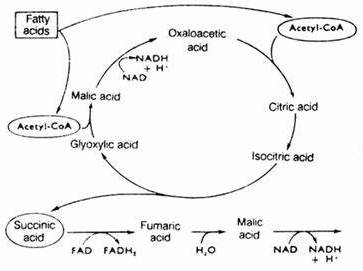
\includegraphics[width=.5\textwidth]{figure/乙醛酸循环.jpeg}
    \end{center}
    \item 乙醛酸循环总反应式:
    \[
        2\text{乙酰CoA}+\text{NAD}^+\to\text{琥珀酸}+2\text{CoA}+\text{NADH}+\text{H}^+
    \]
    \item 植物乙醛酸循环在\uline{乙醛酸循环体}(一种\uline{微体},与过氧化物酶体同源)和\uline{线粒体}中协同进行,可以说是三羧酸循环的辅佐途径。
    \item 动物细胞中没有乙醛酸体,无法将脂肪酸转变为糖。 
    \item 乙醛酸循环在异柠檬酸与琥珀酸、苹果酸间搭了一条捷径。
    \item \textcolor{red}{乙醛酸循环的化学历程:}
    \begin{enumerate}
        \item 脂肪酸在乙醛酸体内经过β-氧化分解为乙酰CoA,后者与\uline{草酰乙酸}缩合为\uline{柠檬酸},进一步形成\uline{异柠檬酸};
        \item 异柠檬酸在异柠檬酸裂解酶的作用下分解为\uline{琥珀酸}和\uline{乙醛酸};
        \item \uline{乙醛酸}与\uline{乙酰CoA}在苹果酸合成酶催化下生成\uline{苹果酸},脱氢形成\uline{草酰乙酸},构成循环;
        \item 琥珀酸由乙醛酸体转移到线粒体参与三羧酸循环,或转移到细胞质生成\uline{磷酸烯醇式丙酮酸(PEP)}参与\uline{糖异生}。(但也有人认为是苹果酸进入的细胞质。)
    \end{enumerate}
    \item \textcolor{red}{乙醛酸循环的作用:}
    \begin{enumerate}
        \item 通过乙醛酸途径使乙酰-CoA转变为草酰乙酸从而进入柠檬酸循环。
        \item 使萌发的种子将贮存的甘油三脂,通过乙酰-CoA转变为葡萄糖。 
    \end{enumerate}
    \item \uline{蓖麻种子}萌发时,乙醛酸循环产物的外运形式是苹果酸,苹果酸或进入细胞质参与糖异生,或通过“\textbf{苹果酸穿梭}”进入线粒体。
    \item 与糖异生的关系:
    \[
        \text{油脂}\overset{\text{β-氧化}}\longrightarrow\text{乙酰CoA}\overset{\text{乙醛酸循环}}\longrightarrow\text{草酰乙酸}\overset{糖异生}\longrightarrow\text{糖}
    \]
\end{enumerate}

\subsection{磷酸戊糖途径}
\begin{enumerate}
    \item \textbf{磷酸戊糖(PPP)途径}:以\uline{6-磷酸葡萄糖}开始,在\textbf{6-磷酸葡萄糖脱氢酶}(限速酶)催化下形成\uline{6-磷酸葡萄糖酸},进而代谢生成\uline{磷酸戊糖}为中间代谢物的过程。
    \item 磷酸戊糖途径总反应式:
    \[
        \text{G-6-P}+12\text{NADP}^++7\text{H}_2\text{O}\to 6\text{CO}_2+12\text{NADPH}+12\text{H}^++\text{H}_3\text{PO}_4
    \]
    \item 磷酸戊糖途径的意义:
    \begin{enumerate}
        \item \uline{产生NADPH},为各种合成反应提供还原力,比如参与脂肪酸和固醇类物质的合成;
        \item 为许多物质的合成提供原料:重要的\uline{5-P-核糖是核苷酸合成的原料};另外比如,\uline{4-P-赤藓糖是氨基酸合成的原料};
        \item 一系列中间产物及酶类与光合作用中卡尔文循环的大多数中间产物和酶相同,因而磷酸戊糖途径可与光合作用联系起来,并实现\uline{某些单糖间的互变}。
        \item 该途径是由葡萄糖直接氧化起始的可单独进行氧化分解的途径,也是\uline{戊糖代谢的主要途径},因此可以和EMP-TCA相互补充、相互配合。
    \end{enumerate}
\end{enumerate}

\section{电子传递链}
\begin{enumerate}
    \item 电子传递链的组成:
    \begin{enumerate}
        \item 复合体I:NADH-泛醌Q还原酶;
        \item 复合体II:琥珀酸-泛醌Q还原酶;
        \item 复合体III:细胞色素还原酶;
        \item 复合体IV:细胞色素氧化酶。
    \end{enumerate}
    \item 电子传递顺序:
    \begin{enumerate}
        \item NAD(P)H氧化呼吸链:NADH$\to$复合体I$\to$Q$\to$复合体III$\to$细胞色素C$\to$复合体IV$\to$O$_2$;
        \item FADH$_2$氧化呼吸链:FADH$_2\to$复合体II¥$\to$Q$\to$复合体III$\to$细胞色素C$\to$复合体IV$\to$O$_2$。
    \end{enumerate}
    \item 电子传递抑制剂:
    \begin{center}
        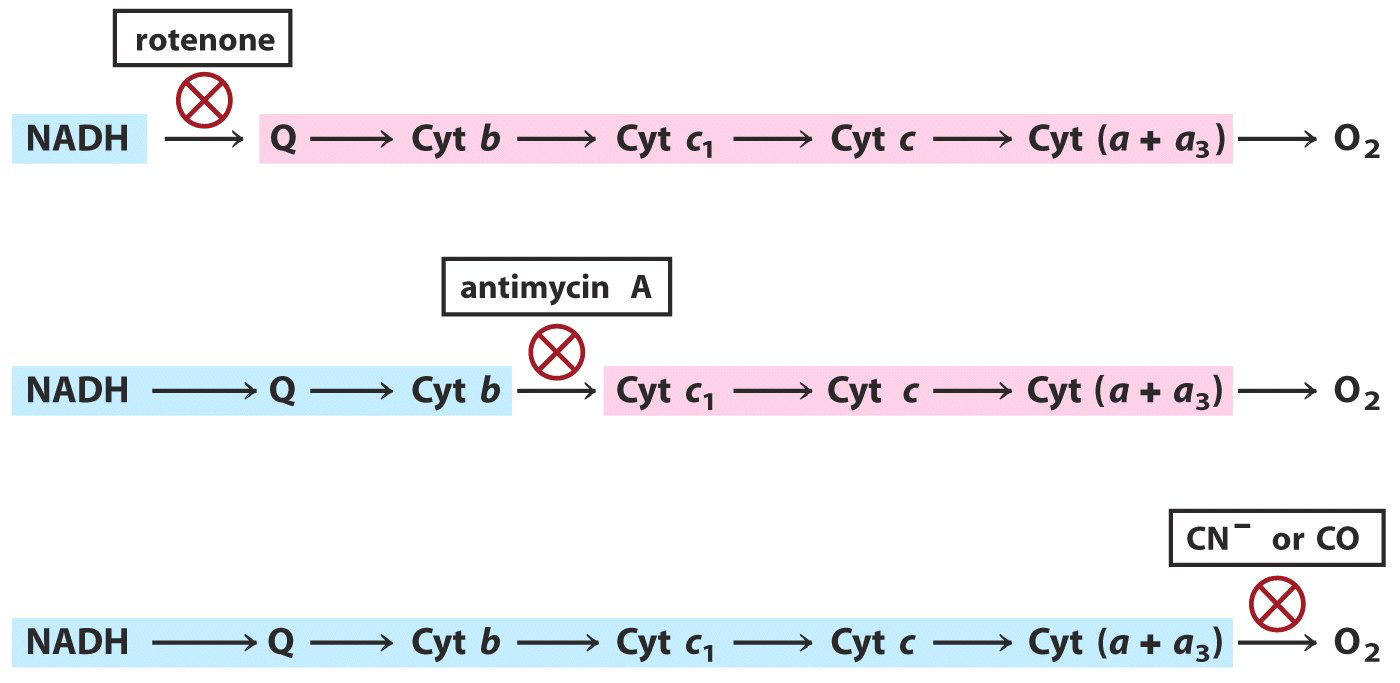
\includegraphics[width=.8\textwidth]{figure/电子传递抑制剂.png}
    \end{center}
\end{enumerate}

\section{氧化磷酸化}
\begin{enumerate}
    \item 底物水平磷酸化:
    \begin{enumerate}
        \item 1,3-二磷酸甘油酸$\overset{\text{3-磷酸甘油酸激酶}}\longrightarrow$3-磷酸甘油酸+ATP;
        \item 磷酸烯醇式丙酮酸$\overset{\text{丙酮酸激酶}}\longrightarrow$丙酮酸+ATP;
        \item 琥珀酰-CoA + H$_3$PO$_4$ + GDP/ADP$\overset{\text{琥珀酰-CoA合成酶}}\longrightarrow$琥珀酸 + CoA + GTP/ATP。
    \end{enumerate}
    \item 电子传递体系磷酸化:末端氧化,有\textbf{能量偶联假说},其下有三个学说:\uline{化学耦联学说}、\uline{结构耦联学说}、\uline{化学渗透学说}。
    \begin{enumerate}
        \item 化学偶联假说:认为电子传递过程产生一种活泼的高能共价中间物。它随后的裂解驱动氧化磷酸化作用。
        \item 构象偶联假说:认为电子传递使线粒体内膜蛋白质组分发生了构象变化,形成一种高能形式。这种高能形式通过ATP的合成而恢复其原来的构象。
        \item 化学渗透学说:认为电子传递释放出的自由能和ATP合成是与一种跨线粒体的质子梯度相偶联的。
    \end{enumerate}
    \item 线粒体外NADH的穿梭:
    \begin{itemize}
        \item 胞液中的3-磷酸甘油醛/磷酸二羟丙酮或乳酸/乙醇脱氢(糖酵解),均可产生NADH。
        \item 这些NADH可经-磷酸甘油穿梭和苹果酸天冬氨酸穿梭两种方式进入线粒体氧化磷酸化过程。
    \end{itemize}
\end{enumerate}

\section{其他末端氧化酶系}
\begin{enumerate}
    \item 抗氰氧化酶系统(线粒体内):有些植物细胞线粒体内存在抗氰氧化酶,当氰化物作用于复合体IV,阻断正常呼吸链时,电子可以从复合体III的Cytb直接传给抗氰氧化酶(绕开细胞色素c和复合体IV细胞色素氧化酶)再交给氧。其生理意义有:
    \begin{enumerate}
        \item 有利于低温地区传粉和种子萌发(放热);
        \item 抵御逆境;
        \item 分流电子:当呼吸底物积累大于生长、储存、ATP合成需要时,通过该途径将多余能量消耗掉。
    \end{enumerate}
    \item 多酚氧化酶系统(线粒体外):此酶与植物组织受伤反应有关,植物组织受伤后多酚氧化酶活力增高,呼吸作用增强;植物受病菌侵害时,多酚氧化酶活力也增高,有利于把酚类化合物氧化为醌,醌对病菌有毒害而起抗病作用。
    \item 抗坏血酸氧化酶系统(线粒体外):可能与植物的抗病有关。
    \[
        \text{抗坏血酸}+\text{O}_2\overset{\text{抗坏血酸氧化酶}}\longrightarrow\text{脱氢抗坏血酸}+\text{H}_2\text{O}
    \]
    \item 超氧化物歧化酶(SOD):清除自由基活性氧,在植物胞质和叶绿体、动物的红细胞和其它细胞、细菌中都存在。
    \item 乙醇酸氧化酶:一种黄素蛋白,存在于过氧化体中,催化乙醇酸氧化为乙醛酸的反应,在光呼吸中起重要作用。此过程中会产生过氧化氢,在过氧化氢酶催化下产生具有强氧化能力的新生态氧,并释放于根的周围,形成一层氧化圈。
\end{enumerate}
\chapter{植物水分关系}
\section{植物细胞水分关系}
\subsection{水势的概念}
\begin{enumerate}
    \item 在植物生理学中,\textbf{水势}($\Psi$)是\uline{每偏摩尔体积水的化学势差(水的化学势差指特定体} \uline{系的水与纯自由水之间的化学势差)}:
    \[
        \text{水势}=\frac{\text{水的化学势差}}{\text{水的偏摩尔体积}(V_w)}
    \]
    \item 物理化学中,体系中某组分的\textbf{化学势}指:\uline{等温等压条件下,在无限大的体系中,加} \uline{入1mol该物质时引起体系自由能的改变量}。化学势的绝对值是不能测定的,通常以给定状态和人为规定的标准状态的差值来表示。
    \item 水势的概念可以理解为体系中的水与纯水之间每单位体积的自由能差。
    \item \textcolor{red}{体系中水势的组分:}
    \[
        \Psi_w=\Psi_s+\Psi_m+\Psi_p+\Psi_g
    \]
    \begin{enumerate}
        \item $\Psi_s$(\textbf{溶质势}):由于\uline{溶质颗粒的存在}而引起体系水势降低的数值,也称\textbf{渗透势}。计算公式:
        \[
            \Psi_s=-iCRT
        \]
        \begin{itemize}
            \item $R$:气体常数(8.31$\text{J}\cdot\text{mol}^{-1}\cdot\text{K}^{-1}$);
            \item $T$:绝对温度(K);
            \item $C$:摩尔浓度($\text{mol}\cdot\text{L}^{-1}$);
            \item $i$:溶解系数。
        \end{itemize}
        \item $\Psi_p$(\textbf{压力势}):由于溶液静水压(膨压)的存在而使体系水势改变的数值。膨压一般为正;但植物细胞中溶液的静水压也可以为负值,如在根、茎部的木质部导管中。同一大气压下,讨论两个开放体系间的水势差时,$\Psi_p$可以忽略不计。
        \item $\Psi_g$(\textbf{重力势}):重力作用使水向下移动,使处于较高位置的水比较低位置的水有高的水势。当体系中的两个区域高度相差不大时,重力势可忽略。
        \item $\Psi_m$(\textbf{衬质势}):亲水的衬质与水的相互作用使水势降低,把这种衬质对水势产生的影响称为衬质势。如干燥的木材、种子等具有很低的$\Psi_m$,可达-300MPa,因此有很强的吸水能力。
    \end{enumerate}
    \item 纯水的水势为0,化学势也为0。
    \item 植物细胞的水势:
    \begin{enumerate}
        \item 无液泡细胞:$\Psi_w=\Psi_m$;
        \item 有液泡细胞:$\Psi_w=\Psi_m+\Psi_p$
    \end{enumerate}
\end{enumerate}

\subsection{水分运动的形式}
\begin{enumerate}
    \item 水分运动的动力是水势差。水分的移动是顺着能量梯度的方向进行的,\uline{水分总是从水势高处移向水势低处,没有任何例外!}
    \item 水分运动的形式:
    \begin{enumerate}
        \item \textbf{扩散}:浓度梯度所推动的物质运动。物质分子(气体、水、溶质分子等)从高浓度区域向低浓度转移,直至均匀分布的现象。叶片气孔蒸腾作用是由植物充满水汽的气孔下腔向水分亏缺的大气扩散水汽的过程;CO$_2$相反。
        \item \textbf{集流}:压力梯度所推动的物质运动。液体中成群的原子或分子在压力梯度下共同移动的现象,与物质浓度无关。水在导管或筛管中的移动是植物体内主要的“集流”水分运动。
        \item \textbf{渗透}:渗透势梯度所推动的水分运动。溶液中的溶剂分子通过半透膜扩散的现象。
    \end{enumerate}
    \item 植物细胞间也可发生水分运动,相邻两个细胞之间水分移动的方向,取决于两细胞间的水势差。
\end{enumerate}
\subsection{细胞吸水的形式}
\begin{enumerate}
    \item 无论哪种吸水方式,推动力都是\uline{水势差}。
    \item 细胞吸水的形式:
    \begin{enumerate}
        \item \textbf{吸胀吸水}:依赖于衬质势的吸水。发生的条件:\uline{有亲水衬质的存在}、\uline{有衬质导致的水势梯度存在}。
        \item \textbf{降压吸水}:因压力势降低而引起的细胞吸水(集流)。细胞压力势经常为正值,很少情况下为负值。\uline{导管}中的压力势为负值,为降压吸水。
        \item \textbf{渗透吸水}:依赖于渗透压的吸水,为植物细胞吸水或脱水的主要动力。高渗环境下,植物细胞脱水时发生质壁分离现象。
    \end{enumerate}
    \item \textbf{水通道蛋白}或\textbf{水孔蛋白}是分子量为25-30KDa、选择性高效转运水分子的膜蛋白。植物细胞膜水通道蛋白能\uline{提高水分传输速率},但\uline{不改变由水势差决定的水分运输方向}。
    \item 质壁分离过程中的水势变化 :
    \begin{enumerate}
        \item 初始质壁分离:$\Psi_p=0$,$\Psi_w=\Psi_s$;
        \item 充分饱和时:$\Psi_w=0$,$\Psi_p=-\Psi_s<0$。
    \end{enumerate}
\end{enumerate}
\subsection{植物组织水势的测定}
\begin{enumerate}
    \item 干湿球温度计:当水溶液的水势降低时水的蒸气压就会降低,表面蒸发量下降,温度升高。相反,较高的水势伴随表面水分蒸发增加,导致表面温度降低。该方法测定慢,但是准确。
    \item 压力室法:认为\uline{木质部溶液的水势}是和植物组织的水势相近的,因此只要测量出木质部溶液的水势,即可得到植物组织的水势。在植物茎切割前,水柱是连续的,处于负压状态;切割后,水柱在负压作用于缩进植物茎;在压力室正压力的作用下,水柱回到切割表面。可室外快速测定,但数据的准确度相对较低。
    \item 冰点下降法:当溶液中溶质浓度上升时,溶液的冰点会下降。测定溶液的冰点温度,可以计算得出溶质势。
    \item 压力探针法:(单细胞膨压测量)玻璃毛细管刺入细胞时,细胞液由于膨压而进入毛细管。推动活塞,使硅油/细胞液界面返回细胞中。这时压力传感器所测出的平衡压力即为膨压值。
\end{enumerate}

\section{植物整体水分平衡}
\subsection{根对水分的吸收}
\begin{enumerate}
    \item 土壤中水分的状态:在大多数情况下土壤中溶质的含量很低,溶质势高,一般 -0.02 MPa,可以忽略不记;盐碱地或干旱条件下,溶质势降低,水势也随之降低。在一般的湿润土壤的条件下,土壤的水势接近纯水的水势。在大多数情况下,土壤的水势是高于植物根水势的。
    \item 按能否被植物利用分为可利用水、不可利用水。区分的指标:\textbf{永久萎蔫系数}。
    \item \textbf{萎蔫}:当植物体内水分亏缺时,植物细胞膨压下降,叶片、幼茎下垂的现象。
    \begin{enumerate}
        \item 暂时萎蔫:当蒸腾速率降低后,萎蔫植物可恢复正常;
        \item 永久萎蔫:蒸腾降低后,萎蔫植物仍不能恢复正常。
    \end{enumerate}
    \item \textbf{永久萎蔫系数}:植物发生永久萎蔫时,土壤中尚存留的水分占土壤干重的百分率,称为永久萎蔫系数,土壤水势称为\textbf{永久萎蔫点}。永久萎蔫系数以上的水为可利用水,以下的水为不可利用水或无效水。
    \item 根吸水的部位:主要在\uline{根顶端}部分,特别是\uline{根毛区(成熟区)}和\uline{伸长区}。
    \item 根毛区吸水能力最强,原因:
    \begin{enumerate}
        \item 根毛增大了吸水面积;
        \item 根毛外壁,果胶质覆盖,亲水性好;
        \item 根毛区输导组织发达,阻力小,水分移动速度快。  
    \end{enumerate}
    \item 水分进入植物的过程:
    \begin{enumerate}
        \item 质外体途径:水分由细胞壁、细胞间隙、胞间层以及导管的空腔组成的质外体部分的移动过程。
        \item 共质体途径:水分依次从一个细胞的细胞质经过胞间连丝进入另一个细胞的胞质的移动过程。
        \item 共质体、质外体交替途径。
    \end{enumerate}
    \item 经表皮和皮层时,水分可以选择质外体还是共质体途径。但无论如何,水分最终必须跨越内皮层的“凯氏带”细胞(纵向壁和横向壁上形成的一条细的木栓质或类木质素的沉积带,细胞壁不透水),即经共质体途径进入木质部导管。所以,理论上说,进入木质部导管的水分均是经共质体过滤的水分。
\end{enumerate}

\subsection{水在植物体内的运输}
\begin{enumerate}
    \item \uline{木质部}是植物体内进行水分运输的主要途径。木质部管部分子:导管和管胞。
    \item 植物\uline{输导组织}有2类结构:导管和管胞,均为死细胞结构,\uline{细胞壁强烈木质化加厚}。许多个\textbf{导管分子}以细胞的两端连接起来就形成了导管。管胞是单个细胞,\uline{端壁没有穿孔},上下连接的管胞靠侧壁上的纹孔传导水分,导水效率低。
    \item 导管:被子植物和一些裸子植物有。管胞:被子植物和裸子植物都有。
    \item 木质部水分向上运输的机制:主动吸水、被动吸水。
    \item \textbf{主动吸水}:指由于\uline{根系的生理活动}引起的吸水过程,与地上部分的蒸腾无关。主动吸水的推力很弱,只有在土壤水分供应充足时才有可能发生。
    \item 主动吸水的证据:吐水、伤流;动力:根压。
    \item \textbf{根压}:由于根系的生理活动产生的促进液流从根部上升的压力。
    \item \textbf{伤流}:土壤水分充足时,一年生植物幼苗在茎基部切断,可以看见切面木质部有液滴流出,持续数小时或更久,这种现象称为伤流。土壤水分充足时,春天修剪后可以观察到多年生树木的伤流。
    \item \textbf{吐水}:在温暖湿润的傍晚或清晨,常可看到植株叶片尖端或边缘排出水滴,这种现象称为吐水。吐水现象在禾本科植物最为常见。
    \item 根压产生的原因:
    \begin{itemize}
        \item 内皮层存在凯氏带;
        \item 根系细胞主动吸收土壤溶液中的离子;
        \item 离子释放进入导管;
        \item 根木质部导管水势下降,根皮层质外体水势高,内皮层内外产生水势差,推动水分吸收,由此产生静水压——根压。
    \end{itemize}
    \item \textbf{被动吸水}:植物根系以\uline{蒸腾拉力}为动力的吸水过程。
    \item \textbf{蒸腾拉力}:指因叶片蒸腾作用而产生的使导管中水分上升的力量。
    \item 解释蒸腾拉力的\textbf{内聚力-张力学说}:
    \begin{itemize}
        \item 内容:植物在顶部的蒸腾作用会产生很大的\uline{负静水压(张力)},这个负压可以将导管的水柱向上拖动形成水分的向上运输。水分子间的\uline{内聚力}保证了木质部水柱的连续性。
        \item 证据:
        \begin{enumerate}
            \item 木质部导管承受着负压(压力室法测定:树木茎干中的负压达到-1.2至-3.5 MPa);
            \item 负压下水柱的完整性:水分子间具有很强的内聚力,水柱可以抵抗-30 MPa的张力,远远高于植物木质部可能的负压;
            \item 导管中的“气穴”栓塞的克服。
        \end{enumerate}
        \item 排除“气穴”的方法:空气难以通过纹孔膜,把气泡阻挡在导管分子或管胞的两端,而水可以通过侧壁的纹孔对进入相邻的导管或管胞。这就维持了水柱的连续性。气泡在蒸腾很弱时会消失。
    \end{itemize}
\end{enumerate}

\section{蒸腾作用}
\begin{enumerate}
    \item \textbf{蒸腾作用}:水从植物地上部分以水蒸汽状态向外界散失的过程称为蒸腾作用。
    \item 蒸腾作用方式:
    \begin{enumerate}
        \item 皮孔蒸腾:茎;
        \item 叶片蒸腾:角质、气孔。
    \end{enumerate}
    \item 不同植物主要蒸腾作用方式不同:
    \begin{enumerate}
        \item 幼小植株:整个植物体(地上部)蒸腾;
        \item 长成植物:以及气孔蒸腾为主;
        \item 水生植物:以角质蒸腾为主;
    \end{enumerate}
    \item 蒸腾作用的指标:
    \begin{enumerate}
        \item \textbf{蒸腾速率}:植物在单倍时间内单倍面积通过蒸腾作用所散失的水量,也叫\textbf{蒸腾强度}(g$\cdot$m$^{-2}\cdot$h$^{-1}$)。
        \item \textbf{蒸腾系数}:植物光合作用固定每摩尔的CO$_2$所需蒸腾散失的水的量。
    \end{enumerate}
    \item 蒸腾速率的测定:
    \begin{enumerate}
        \item 称重法:离体器官快速称重,测植株重量变化。
        \item 气量计:测定相对湿度的短期变化。
        \item 红外线分析仪:测定温度变化。
    \end{enumerate}
    \item 气孔蒸腾是陆生植物在进化过程中形成的解决CO$_2$吸收和水分蒸发之间矛盾的一个有效机制。
    \item 不同植物叶片的气孔分布:
    \begin{enumerate}
        \item 双子叶植物:主要在下表皮;
        \item 单子叶植物:上下表皮;
        \item 木本植物:只分布在下表皮;
        \item 水生植物:只分布在上表皮。
    \end{enumerate}
    \item \textbf{气孔复合体}:保卫细胞、副卫细胞或邻近细胞以及保卫细胞中的小孔。
    \item 保卫细胞的类型:
    \begin{enumerate}
        \item \textbf{肾形保卫细胞}(有或没有副卫细胞)的\uline{内壁(靠气孔一侧)厚而外壁薄},\uline{微纤丝从气孔呈扇形辐射排列}。当保卫细胞吸水膨胀时,较薄的外壁易于伸长,向外扩展,但微纤丝难以伸长,于是将力量作用于内壁,把内壁拉过来,于是气孔张开。
        \item \textbf{哑铃型保卫细胞}(有副卫细胞)\uline{中间部分的胞壁厚,两头薄},\uline{微纤丝径向排列}。当保卫细胞吸水膨胀时,微纤丝限制两端胞壁纵向伸长,而改为横向膨大,这样就将两个保卫细胞的中部推开,于是气孔张开。
    \end{enumerate}
    \item 气孔运动的动力:保卫细胞的吸水膨胀或失水收缩。
    \item 气孔开放时间: 白天开放晚上关闭;CAM(景天酸代谢)途径植物白天关闭,晚上开放。
    \item 外界环境因素对气孔运动的影响:
    \begin{enumerate}
        \item 光照:光照下张开,黑暗下关闭;
        \item CO$_2$:低浓度CO$_2$导致气孔张开;
        \item 空气湿度:水分亏缺时气孔关闭;
        \item 温度:高温导致气孔关闭或开放;
        \item 风:风使气孔关闭,间接作用。
    \end{enumerate}
    \item 气孔运动的内在调节机制:
    \begin{enumerate}
        \item 气孔运动的渗透调节机理:通过改变渗透势和膨压实现,渗透调节机制是基础调节机制。
        \item 在蓝光照射下气孔扩大:依赖于保卫细胞的光合作用;被蓝光和红光信号系统所推动。  
        \item ABA对气孔运动的调节:水分亏缺诱导保卫细胞内外ABA浓度升高,引起气孔关闭。
    \end{enumerate}
    \item 渗透调节机理的三种学说:
    \begin{enumerate}
        \item 质子泵假说:光激活保卫细胞策膜H$^+$-ATPase,$H^+$泵出,保卫细胞pH升高,内向$K^+$通道打开,K$^+$进入保卫细胞(伴随Cl$^-$进入),水势降低,水分进入,气孔张开。(ABA正好相反)
        \item 苹果酸代谢假说:光导致保卫细胞内CO$_2$消耗,pH升高,活化PEP羧化酶,促进淀粉降解为PEP,PEP与CO$_2$生成草酰乙酸,被NADPH还原为苹果酸,水势降低,水分进入,气孔张开。
        \item 蔗糖-淀粉假说:淀粉转化为蔗糖导致水势降低,水分进入,气孔张开。
    \end{enumerate}
    \item 气孔的运动可能有不同的渗透调节阶段:
    \begin{enumerate}
        \item 日出时光照引起的气孔张开阶段,保卫细胞对钾离子的吸收是主要的渗透调节机制;
        \item 日出后保卫细胞的蔗糖浓度逐渐提高,成为主要的渗透物质。
    \end{enumerate}
    \item 蓝光诱导气孔开放的机制:
    \begin{itemize}
        \item \uline{蓝光紫外光受体向光素}自我磷酸化而激活,诱导保卫细胞内\uline{钙浓度变化},激活H$^+$-ATPase;
        \item 红光受体光敏色素和蓝光紫外光受体隐花色素也参与了气孔开放调节。
    \end{itemize}
    \item 蒸腾作用的意义:
    \begin{enumerate}
        \item 蒸腾拉力是植物吸收水分与传导水分的动力;
        \item 调节植物体温;
        \item 促进木质部内溶液中物质的运输;
        \item 蒸腾作用的正常进行有利于CO$_2$吸收和同化。            
    \end{enumerate}
\end{enumerate}
\chapter{植物的矿质营养}
\section{植物体内的必需元素}
\begin{enumerate}
    \item 将植物组织在100-105度下烘干,留下干物质(占5-90\%)。将干物质在600度下灼烧,部分元素(C、H、O、N和部分S)在燃烧时挥发。灼烧后剩下的固体残留物称为灰分,灰分中含有的元素称为\textbf{灰分元素},也叫\textbf{矿质元素},包括小部分S、全部P(非金属元素,以矿物质的硫酸盐、磷酸盐形式存在)和所有金属元素。\uline{把N也归入矿质元素中。}
    \item 不同植物灰分含量不同:盐生植物>中生植物>水生植物。
    \item 不同组织器官灰分含量不同:叶>根茎>种子>木质部。
    \item 植物必需元素的确定方法:\uline{不可缺少性}、\uline{不可替代性}、\uline{直接功能性}。
    \item 17种植物必需元素:
    \begin{enumerate}
        \item 9种大量元素:C、H、O、N、P、K、Ca、Mg、S;
        \item 8种微量元素:Cl、Fe、B、Mn、Zn、Cu、Ni、Mo。
    \end{enumerate}
    \item \textcolor{red}{植物主要必需元素的生理功能:}
    \begin{enumerate}
        \item N:组成细胞质、细胞核、细胞壁,是构成生命体各类化合物的元素。N过多,叶色深绿,营养体徒长,抗逆能力差。N过少,植株小,叶色淡,籽粒不饱满,产量低。
        \item P:四大生命分子代谢。缺磷导致植物生长受阻,且由于糖分运输受阻,叶片中积累大量糖分,易形成花色素苷,导致叶色暗绿。
        \item K:调节细胞渗透势,提高原生质水合程度;促进物质合成和代谢,作为60多种酶的泛化剂;促进能量代谢;促进物质运输;与淀粉和纤维素的形成有关,抗倒伏。
        \item Ca:细胞的重要结构成分,组成细胞壁的果胶钙,是磷脂与蛋白质间的桥梁;细胞内的第二信使;酶的活化剂;与抗病有关,促进受伤部位形成愈伤组织;结合草酸以消除毒害。
        \item Fe:呼吸链和光合链中酶的辅基;叶绿素合成需要;固氮酶的成分。(吸收形式为Fe$_2$O$_3$。)
        \item Zn:色氨酸合成酶的必要成分;叶绿素合成需要。
        \item Ni:脲酶的必需组分。
    \end{enumerate}
\end{enumerate}

\section{植物对矿质元素的吸收及运输}
\begin{enumerate}
    \item 水和营养离子吸收部位:根顶端部分,特别是\uline{根毛区(成熟区)}。
    \item 根系吸收矿质元素的过程和途径:
    \begin{enumerate}
        \item 土壤溶液中多数以离子形式存在的矿质元素先通过\uline{离子交换}或\uline{接触交换}被吸附在根组织表面;
        \item 自由扩散进入根内部自由空间;
        \item 经质外体或共质体途径到达内皮层;
        \item 经共质体途径穿越内皮层细胞,进入根组织维管束的木质部导管。然后,随木质部汁液在蒸腾拉力和根压的共同作用下上运至植物的地上部分。
    \end{enumerate}
    \item 根系吸收矿质营养与吸收水分的关系:相互联系,相对独立。
    \begin{itemize}
        \item 相互联系:
        \begin{enumerate}
            \item 矿质营养元素只有溶于水才能被植物吸收;
            \item 活细胞对矿质元素的吸收导致细胞水势降低,促进细胞吸水。
        \end{enumerate}
        \item 相对独立:
        \begin{enumerate}
            \item 水分子和矿质元素通过不同的跨膜转运蛋白进行跨膜吸收;
            \item 细胞对水分和矿质元素的吸收不成比例;
            \item 动力:水分吸收动力是\uline{蒸腾拉力},矿质元素的吸收动力是\uline{代谢能量};
            \item 运输去向:水分运输至叶片,矿质元素运输到生长中心。
        \end{enumerate}
    \end{itemize}
    \item 根系对离子吸收具有选择性:
    \begin{enumerate}
        \item \textbf{生理酸性盐}:如硫酸铵,铵离子吸收大于硫酸根离子,伴随根细胞释放氢离子,使环境酸化。
        \item \textbf{生理碱性盐}:如硝酸钠或硝酸钙,硝酸根离子吸收大于阳离子,并伴随氢离子吸收,使环境碱化。
        \item \textbf{生理中性盐}:如硝酸铵,阴阳离子平衡吸收,不会改变土壤pH。
    \end{enumerate}
    \item \textcolor{red}{\textbf{单盐毒害}}:若将植物培养在某一单盐溶液中,即使浓度很低(低于正常情况下受害浓度),不久即呈现不正常状态,最后枯死。原因是当培养在仅含有一种盐类溶液中的植物,将很快的积累离子。
    \item \textcolor{red}{\textbf{离子拮抗}}:若在单盐溶液中加入少量其他盐类,单盐毒害即可消除。
    \item 要使植物生长良好,必须使其在含有适当比例的多盐溶液中生长,这种能使植物正常生长的混合溶液称为\textbf{平衡溶液}。对于海生植物来说,海水就是其平衡溶液,陆生植物,土壤溶液一般就是其平衡溶液。
    \item 影响根系吸收矿质元素的主要因素:
    \begin{enumerate}
        \item 土壤温度:存在最适温度;
        \item 通气状况:O$_2$较多时吸收旺盛,CO$_2$过高时抑制吸收;
        \item 土壤溶液浓度:存在饱和吸收速率;
        \item 土壤pH:酸性环境有得于阴离子吸收,碱性环境有利于阳离子吸收,但极端pH都不利于矿质吸收。
    \end{enumerate}
    \item 除根以外,植物地上部分也可以吸收矿质营养,这一过程称为\textbf{根外营养}。地上部分吸收矿物质的器官主要是叶片,所以也称为\textbf{叶片营养}。通过\uline{气孔、皮孔、角质层}吸收。
    \begin{itemize}
        \item \textbf{角质层}:多糖和角质的混合物,其上有裂缝,呈细微的孔道。
        \item \textbf{外连丝}:贯穿植物表皮细胞外侧壁的一种胞间连丝样纤细通道,可能起源于胞间连丝。从胞内或质膜延伸到胞壁表面,可能是细胞内、外间物质交流的途径之一。
        \item 根外吸收途径:溶液$\to$角质层孔道$\to$表皮细胞外壁$\to$外连丝$\to$表皮细胞的质膜$\to$细胞内部。
    \end{itemize}
    \item 矿质元素在体内的运输:
    \begin{itemize}
        \item 形式:N为有机物,其他元素为无机盐;
        \item 途径:根吸收的矿质元素由\uline{木质部导管}向上运输、横向运输;叶片吸收的矿质元素由\uline{韧皮部}向下运输、横向运输。
    \end{itemize}
    \item 矿质元素的循环利用:
    \begin{enumerate}
        \item 可再利用元素:在植物体内可反复多次的被利用,如N、P、K、Mg、Cl;
        \item 不可再利用元素:在植物体内形成稳定的化合物,不易移动,不易被循环利用,如Fe、S、Ca、Mn、B。
    \end{enumerate}
\end{enumerate}

\section{植物细胞跨膜离子运输机制}
\begin{enumerate}
    \item 离子跨膜运输蛋白:离子通道、离子载体、离子泵。
    \item 离子载体运输的物质:矿质营养元素离子、呈离子状态的有机代谢物(例如一些氨基酸、有机酸)。
    \item 植物细胞膜上确认的离子泵:
    \begin{enumerate}
        \item 质膜上的H$^+$-ATP酶和Ca$^{2+}$-ATP酶;
        \item 液泡膜上的H$^+$-ATP酶和Ca$^{2+}$-ATP酶;
        \item 内膜系统上的$H^+$-焦磷酸酶。
    \end{enumerate}
    \item \textbf{初级主动运输}:植物细胞膜上由 H+-ATP 酶所执行的主动运输过程。
    \item \textbf{次级主动运输}:由 H+-ATP 酶活动所建立的跨膜质子电化学梯度所驱动的其他无机离子或小分子有机物质的跨膜运输过程。次级主动运输是协同运输过程,即两种离子同时被跨膜运输的过程,分为同向和反向运输两个不同的过程。要把某种有害的离子(如Na$^+$)逆浓度梯度主动排出细胞,是反向共运输。
\end{enumerate}
\chapter{韧皮部运输与同化物分配}
\section{韧皮部结构和运输特点}
\begin{enumerate}
    \item \uline{韧皮部}是同化物运输的主要途径。同化物在韧皮部中可向上、向下运输,运输的方向取决于库(生长中心)的位置。
    \item 韧皮部的结构:韧皮部在维管组织的向外一侧,主要由\uline{筛分子}、\uline{伴胞}和\uline{薄壁细胞}组成,在维管束的外周常包围着一层鞘,称\textbf{维管束鞘}。
    \item 单子叶植物和双子叶植物维管束差异:
    \begin{enumerate}
        \item 单子叶植物:维管束多独立分布于基本组织间。一年生禾本科植物只有初生结构,没有次生结构。
        \item 双子叶植物:连成一环。多年生树木初生结构消失,只有次生韧皮部和次生木质部。
    \end{enumerate}
    \item \textbf{筛分子}是筒状细胞,有线粒体和滑面内质网,有完整质膜。但是\uline{没有细胞核}。筛管分子组成筛管。筛管分子的壁上形成多孔的特化筛域——\textbf{筛板}。
    \item \textbf{伴胞}:在筛管周围,通常具有浓厚的细胞质、大量的线粒体,有细胞核。在筛管分子和伴胞之间有大量的胞间连丝。
    \item 伴胞的RNA和蛋白质可以运输到无细胞核的筛分子中,可能指导筛分子的功能。由于筛管分子和伴胞之间在结构和功能上的密切联系,通常把两者作为一个功能单位看待,称为\textbf{筛管分子-伴胞复合体(SE-CC complex)}。
    \item 韧皮部薄壁细胞:与其他组织中的薄壁细胞类似,细胞壁较薄,液泡很大,但是通常比普通薄壁细胞更长一些。可能有溶质和水的储存和运输的功能。
    \item 韧皮部运输的物质:水、干物质(非还原糖、含氮有机物、无机离子)。
    \item 韧皮部运输的方向:\uline{从源到库}。源:指生产同化物以及向其他器官提供营养的器官,如成熟叶片、种子萌发时的子叶或胚乳组织。库:消耗或积累同化物的接纳器官,如幼叶、根、花、果实、种子等。
    \item \textbf{源库单位}:同化物供求上有对应关系的源与库称为源-库单位。植物体内存在多源多库,同化物在源库器官中的运输存在空间和时间上的调节和分工。
    \item 源库间运输的规律:
    \begin{enumerate}
        \item 空间上就近运输;
        \item 优先在有维管束相连的源库间运输(维管束的并接:当维管束因植物受到伤害或修剪被切断时,韧皮部运输会发生改变);
        \item 向生长中心运输。
    \end{enumerate}
\end{enumerate}

\section{压力流动学说}
\begin{enumerate}
    \item \textcolor{red}{压力流动学说的内容:}
    \begin{itemize}
        \item 源端装载:在源端韧皮部进行溶质的装载$\to$溶质分子进入筛管分子$\to$细胞渗透压下降$\to$水势下降$\to$木质部的水顺着水势梯度进入筛管分子$\to$源端筛管分子膨压上升。
        \item 库端卸载:在库端韧皮部进行溶质的卸出$\to$溶质分子流出筛管分子$\to$细胞渗透压上升$\to$水势上升$\to$筛管的水顺着水势梯度流出,进入木质部$\to$库端筛管分子膨压下降。
    \end{itemize}
    \item 动力来源:源端(膨压高)到库端(膨压低)的膨压梯度推动韧皮部液流运动。
    \item 溶质在筛管中是随\uline{集流}而运动的,筛管内的集流是靠源端和库端渗透势引起的膨压差所建立的压力梯度来推动的。
    \item 压力流动学说的要点:
    \begin{enumerate}
        \item 同化物在筛管内运输是由源、库两侧筛管分子-伴胞复合体内渗透作用所形成的\uline{压力势梯度}所驱动的。
        \item 压力梯度的形成则是由于源端光合同化物不断向筛管分子-伴胞复合体进行装载,库端同化物不断从筛管分子-伴胞复合体卸出,以及韧皮部和木质部之间水分的不断再循环所致。
        \item 只要源端光合同化物的韧皮部装载和库端光合同化物的卸出过程不断进行,源、库间就能维持一定的压力梯度,在此梯度下,光合同化物可源源不断地由源端向库端运输。
        \item 在韧皮部的运输系统中,\uline{筛板极大的增加了筛管对水流的阻力},这种阻力对建立和维持源-库两端的膨压差是必须的。
    \end{enumerate}
\end{enumerate}

\section{韧皮部源端装载和库端卸出机制}
\subsection{韧皮部源端的装载}
\begin{enumerate}
    \item 韧皮部的装载:包括光合产物从成熟叶片中的\uline{叶肉细胞的叶绿体}运送到\uline{筛管分子-伴胞复合体}的整个过程。
    \item 韧皮部装载的步骤:
    \begin{enumerate}
        \item 光合作用中形成的\uline{磷酸丙糖}从叶绿体运到细胞质中,转化为\uline{蔗糖}。
        \item 蔗糖从叶肉细胞转移到叶片小叶脉筛管分子附近。这一途径的距离通常为2-3个细胞直径,称为\textbf{短距离运输途径}。
        \item 蔗糖转运到筛管分子中,称为\textbf{筛管分子装载}。
    \end{enumerate}
    \item 蔗糖及其他溶质进入筛管后,会随集流运出源器官,这个过程称之为\textbf{输出}。
    \item 从源经过维管系统到库的运输称为\textbf{长距离运输},由源库之间筛分子膨压差所推动。
    \item \textcolor{red}{共质体途径和质外体途径:}
    \begin{enumerate}
        \item 共质体途径:整个途径的细胞间都具有胞间连丝。
        \item 质外体途径:质外体途径并不意味着全过程都是在质外体中进行,只要在此途径中任何步骤必须经过质外体,那么这个途径就是质外体途径的韧皮部装载。
    \end{enumerate}
    \item 韧皮部装载类型的决定因子是细胞间是否存在共质体通道。筛管分子-伴胞复合体与周围细胞间胞间连丝的密度:
    \begin{enumerate}
        \item 有大量胞间连丝存在——共质体装载;
        \item 有中等密度的胞间连丝存在——共质体/质外体装载);
        \item 几乎无胞间连丝——质外体装载。
    \end{enumerate}
    \item 蔗糖可采取质外体途径或共质体途径,而棉子糖、苏水糖只采取质外体途径。
    \item 质外体途径的韧皮部装载机制:
    \begin{itemize}
        \item 质外体途径的蔗糖装载是需能的过程。
        \item 蔗糖/质子共转运蛋白:运输蔗糖与质子传递相偶联。 筛分子/伴胞质膜上的H$^+$-ATP酶产生电化学势梯度,推动载体将H$^+$的向内扩散与蔗糖的向共质体的转运偶联起来,称为\textbf{蔗糖/质子共转运}。属于\uline{次级主动运输}。
        \item 实际上,在筛分子-伴胞复合体装载前,必须从叶肉细胞中卸出。卸出的跨膜机制目前还是未知。
    \end{itemize}
    \item 共质体途径的韧皮部装载机制:共质体途径装载是通过胞间连丝进行的,是一种\uline{由浓度梯度推动}的装载。所以,细胞间存在胞间连丝是共质体运输的必要条件。
\end{enumerate}
\subsection{韧皮部库端的卸出}
\begin{enumerate}
    \item \textbf{韧皮部卸出}:韧皮部进行输出的同化物在库端被运出韧皮部并被邻近生长或储存组织所吸收的过程。
    \item 韧皮部输出过程也分为质外体和共质体路径。
    \item 植物器官发育过程中可能发生装载和卸出的转换。例如,幼小的叶片是接收同化物的库,在叶片发育的过程中逐步转化为源。
    \item 卸出途径的研究手段:
    \begin{enumerate}
        \item CFDA:不发荧光,非极性,可跨膜进入活细胞。进入活细胞后经非特异酯酶分解为CF,发荧光,极性分子,不能跨膜泄漏。
        \item 病毒运动蛋白+荧光蛋白:进入细胞后经胞间连丝在活细胞中运动。
    \end{enumerate}
    \item 葡萄果实发育前期果实中糖浓度很低,韧皮部采用共质体卸载路径可能有利于浓度梯度推动的卸出。而果实始熟后糖迅速积累,这时韧皮部质外体卸载有利于果实中逆浓度积累糖。
\end{enumerate}

\section{同化物的配置和分配}
\begin{enumerate}
    \item 植物将光合固定的碳调配到不同代谢途径称为\textbf{配置}。同化物配置与源叶输出和库器官同化物积累分配直接相关联。
    \item 光合叶片中同化物的配置:
    \begin{enumerate}
        \item 储存:光合固定的碳用于\uline{合成储存化合物}:大多数植物白天在叶绿体中合成和储存淀粉,夜间淀粉被动员用于输出。
        \item 利用:光合固定的碳可以\uline{被光合细胞自身所利用}。
        \item 运输:光合固定的碳\uline{合成用于运输的糖},然后被运输到各种库组织中。
    \end{enumerate}
    \item 库中的配置:储存、利用。
    \item 配置的调节:源叶中同化物配置的控制点是\uline{磷酸丙糖}配置。磷酸丙糖有三个去向:加入光合C3循环、进行淀粉合成、进行蔗糖合成。蔗糖合成过程中的关键酶是蔗糖磷酸合成酶和果糖-1,6-二磷酸酶。叶绿体淀粉合成中的关键酶是ADPG焦磷酸化酶(催化ADPG合成),这些酶是协调淀粉和蔗糖合成的控制点,也是源叶中同化物配置的关键调节点。这些代谢节点的调节(同化物配置调节)与源叶输出和库器官同化物积累分配直接相关联。
    \item 植物体中光合同化物有规律地向各库器官输送的模式称为\textbf{分配}。同化物的分配直接影响到植物生长和经济产量。
    \item 同化物分配的影响因素:源库间距离、维管束走向、横截面积及库器官的竞争能力。
    \item 库器官的类型:
    \begin{enumerate}
        \item \textbf{使用库}:是指大部分输入的同化物被用于生长的组织。在大部分使用库中,韧皮部与周围细胞有较多的胞间连丝,韧皮部的卸出通常采用共质体的途径。由于库细胞中同化物被不断代谢利用,可以保持韧皮部细胞与库细胞之间从高到低的同化物浓度差,有利于浓度梯度推动的共质体卸载。
        \item \textbf{储藏库}:是指大部分输入的同化物用于储藏的组织和器官,如果实、块茎、块根等。在许多储藏库中,韧皮部与周围细胞间有许多胞间连丝存在,韧皮部筛管分子卸出以共质体途径为主,随后的筛管分子后运输过程中经历了同化物卸出到质外空间,再通过质外体装载进入库细胞的过程。这实际上是一种质外体卸出路径。
    \end{enumerate}
    \item 库器官对同化物的竞争能力可能决定了植物体内同化物的分配。库的储藏和代谢输入糖的能力越强,从源争夺同化物的能力也就越强。这种竞争决定了运输糖在各种库组织间的分配。
    \item 库对同化物的竞争能力用\textbf{库强度}表示。
    \[
        \text{库强度}=\text{库容量}\times\text{库活力}
    \]
    \begin{itemize}
        \item \textbf{库容量}:库组织的总量;
        \item \textbf{库活力}:单位库组织吸收同化物的速率。
    \end{itemize}
    \item 库源的协调:
    \begin{enumerate}
        \item 源是库的供应者。源强会为库提供更多的光合产物。
        \item 库对源有反馈调节作用库强则能促进源中蔗糖的输出速率,并促进源叶光合速率。库弱抑制同化物输出,抑制叶片光合作用。库小源大:限制光合产物的输送分配,抑制光合作用。库大源小:促进光合作用,但当库的需求远超过源的负荷时,导致\uline{胁迫输送},引起库的空瘪和叶片早衰。
        \item 源库之间的信号传递:通过植物激素。糖水平影响光合作用和糖代谢有关基因的表达。糖不足,促进光合作用、储藏物动员输出有关基因的表达;糖富足,促进与储藏利用碳水化合物有关基因的表达。
    \end{enumerate}
    \item 同化物的\textbf{再分配}:植物体内已经同化的物质,除了已构成细胞壁这样的骨架物质外,其他物质——不论是有机的还是无机的——都可进行再度分配和再度利用。
    \item 同化物再分配的途径是\uline{韧皮部}。
\end{enumerate}
\chapter{植物的生长发育}
\section{植物细胞生长分化}
\begin{enumerate}
    \item \textbf{植物生长发育}:从受精卵发育开始,形成植物个体的整个过程。
    \item \textbf{植物生长发育周期}:从受精卵发育开始,形成植物个体,最后形成雌/雄配子体,可以称作一个发育周期。
    \item \textbf{生长}:指植物器官在体积、重量、数目等形态指标方面的增加,是一种量的变化。细胞水平上是通过原生质的增加,细胞分裂、伸长和扩大来实现的。整株水平上是根,茎,叶,花,果实和种子的体积增大和干重的增加。
    \item \textbf{发育}:是植物生长和分化的动态过程与总和。
    \begin{enumerate}
        \item 叶的发育:叶原基分化到长成成熟的叶片。
        \item 根的发育:根原基的发生到形成完整根系。
        \item 花的发育:茎端的分生组织形成花原基,转变成花蕾,到形成花序最后花蕾长大。
    \end{enumerate}
    \item 植物细胞分裂:末期由高尔基体分泌的小泡形成的细胞板实现细胞质分裂。
    \item 植物细胞分化过程四步模式:信号产生和感受$\to$分化调节基因表达$\to$结构和功能基因表达$\to$结构和功能分化成熟。
    \item 植物细胞分裂分化的特点:全能性。
\end{enumerate}

\section{植物发育——从胚胎到整体}
\subsection{高等植物生长发育的特点}
\begin{enumerate}
    \item \textbf{分生组织}:植物体内的一些体积较小、等直径的胚性细胞。
    \item \textbf{组织原细胞}:分生组织内衍生各种组织的原始细胞。
    \item 分生组织“自我存留”的性质:分裂的两个细胞,一个保留组织原细胞的特性,另一个进入特定分化进程。
    \item 分生组织的分类
    \begin{enumerate}
        \item \textbf{初生分生组织}:在胚胎发育过程中形成的分生组织,包括根和茎的顶端分生组织,以及侧生分生组织:原表皮层(分化形成表皮组织)、基本分生组织(分化形成皮层和内皮)和原形成层(分化形成维管组织和中柱鞘)。在多年生植物中仅存根和茎的顶端分生组织。
        \item \textbf{次生分生组织}:后期发育过程中形成的分生组织,包括叶腋分生组织、侧生分生组织中的维管形成层和表皮形成层,以及禾本科植物节间基部居间分生组织。
    \end{enumerate}
    \item 次生分生组织与初生分生组织在构造和性质上完全相同。
    \item 植物生长的有限性和无限性:
    \begin{enumerate}
        \item \textbf{有限性}:植物的组织器官到一定的阶段和大小时就停止生长发育,然后衰老、死亡。植物的叶片,花,果实等器官;
        \item \textbf{无限性}:营养器官的生长具有潜在的无限性,根,茎等器官。
    \end{enumerate}
    \item 植物的一年生和多年生习性:
    \begin{enumerate}
        \item 单次结实性:只开一次花,然后衰老死亡;
        \item 多次结实性:多年生植物在每次开花结实时,仍然保留大量的营养枝。
    \end{enumerate}
\end{enumerate}
\subsection{植物生长发育的控制}
\begin{enumerate}
    \item 基因水平的控制:胞内细胞信号过程,转录水平,转录后水平,翻译和翻译后水平;植物生长发育是基因程序性表达的结果。
    \item 激素水平的控制:胞间细胞通讯、胞内信号转导、基因表达调节。
    \item 环境的控制:胞外信号:光、温、水、重力、磁场、风、土壤的酸碱度,等。细胞接受环境信号,通过细胞内信号转导,调节基因表达,控制生长发育进程。
    \item 环境和激素最终通过调节基因表达来控制生长发育。
\end{enumerate}
\subsection{植物胚胎发育}
\begin{enumerate}
    \item \textbf{胚胎发生}:植物的生长发育是从\uline{子房胚囊}内的单细胞受精卵发育为多细胞胚胎这个过程开始的。
    \item \textbf{植物发育基本格式}:植物整体的轴向构造格式和器官径向构造格式。
    \begin{enumerate}
        \item \textbf{轴向构造格式}(整体):植物体呈现根茎两极模式,这种形态特点是植物极性构造的表现。
        \item \textbf{径向构造格式}(器官):根或茎的横截面各种组织呈现典型的同心圆排列形态:表皮,皮层,内皮层,中柱鞘和中柱。
    \end{enumerate}
    \item \textcolor{red}{胚胎发育的三个阶段}:
    \begin{enumerate}
        \item \textbf{球形胚}:\uline{轴向两极已经确定},并\uline{表现出径向构造格式}。
        \item \textbf{心形胚}:\uline{轴向构造已经形成}。
        \item \textbf{鱼雷形胚}:径向构造、轴向构造\uline{全部形成}。
    \end{enumerate}
\end{enumerate}
\subsection{种子的萌发}
\begin{enumerate}
    \item 种子是由\uline{受精胚珠}发育而来的,是脱离母体的延存器官。
    \item 严格地说,生命周期是从受精卵分裂形成胚开始的,但人们习惯上还是以种子萌发作为个体发育的起点,因为农业生产是从播种开始的。
    \item 双子叶植物:胚乳退化,子叶储藏营养。
    \item 单子叶植物:有胚乳。
    \item 通常以\uline{胚根突破种皮}作为萌发的标志。根据萌发过程中种子吸水量,即种子鲜重增加量的“快-慢-快”的特点,可把种子萌发分为三个阶段。
    \item 种子萌发过程中,酶系统形成,ABA减少,GA和IAA增加。
    \item 种子萌发的类型:
    \begin{enumerate}
        \item 子叶出土型:下胚轴伸长将子叶推出土,如蚕豆;
        \item 子叶留土型:上胚轴伸长,如菜豆、单子叶植物;
    \end{enumerate}
\end{enumerate}
\subsection{根系的生长分化}
\begin{enumerate}
    \item 根的结构特点:结构类型相同的组织细胞呈条状排列。从外到内:\uline{表皮-皮层-内皮层-中柱鞘-中柱}。
    \item 根中的所有组织都是从根尖分生组织中分裂产生的组织原细胞衍生而来。
    \item \textbf{静止中心}是根的干细胞群,可以自我更新,其功能在于维持或更新其周围的组织原细胞。
    \item 各种组织的原细胞分裂产生相应的组织:
    \begin{enumerate}
        \item 根冠柱原$\to$根冠柱;
        \item 根冠表皮原$\to$侧根冠和表皮;
        \item 皮层内皮层原$\to$皮层和内皮层;
        \item 中柱原$\to$中柱鞘和中柱。
    \end{enumerate}
    \item 根尖分生区的分裂:
    \begin{enumerate}
        \item 分化分裂:一般为平周分裂,形成条状组织的基础;
        \item 增殖分裂:一般为垂周分裂,增加条状组织的细胞数目。
    \end{enumerate}
    \item 侧根分化:中柱鞘或内皮层(因植物种而异)产生侧根原基,进而分化形成侧根。
\end{enumerate}
\subsection{茎的生长分化}
\begin{enumerate}
    \item 茎尖细胞的分化:茎尖产生许多侧生结构,包括叶原基、芽原基、花器官原基等。
    \item 原套原体理论:
    \begin{itemize}
        \item 原套和原体称为\textbf{组织形成层}。
        \item 表面一至数层排列整齐、较小的细胞为原套,进行垂周分裂,使茎尖的表面积增大。
        \item 原体细胞较大,可进行各个方向的分裂,使茎尖的体积增大。
    \end{itemize}
    \item 中央区周缘区理论:
    \begin{itemize}
        \item 中央区:中央母细胞区,细胞大,分裂慢。它产生茎中所有组织的原细胞。
        \item 中央区下——肋状分生区:分化为茎的内部组织(皮层、内皮和中柱)。
        \item 周缘区:细胞体积小,分裂快。形成叶、腋芽和茎的外层。中央区周缘区包含了原套和原体。
    \end{itemize}
    \item 茎分生组织分为:
    \begin{enumerate}
        \item 营养分生组织:分化叶片,腋芽,和维持茎尖无限生长;
        \item 成花分生组织:分化花器官原基(萼片,花瓣,雌蕊,雄蕊)。
    \end{enumerate}
\end{enumerate}
\subsection{叶的生长分化}
\begin{enumerate}
    \item 叶原基的形成及其分化:\textbf{叶原基}是顶端分生组织原套L1和L2层局部细胞(周缘分生组织区)分裂产生的。子细胞经平周分裂,突出表面形成叶原基,同时叶原基表层细胞进行垂周分裂增加表面积。 
    \item 叶原基的发生并不是随机的,在时间和空间上具有相当的确定性和精确性,并且叶原基发生形态具有种属特异性。叶原基或叶片在茎干上特定的排列状态称为\textbf{叶序}。叶片形态和叶序是植物分类的重要依据之一。
    \item 叶原基分裂分化产生叶片,叶片划分为
    \begin{enumerate}
        \item 近轴区:叶片上表面、朝向顶端分生组织中心的一面;
        \item 远轴区:叶片下表面、背向顶端分生组织中心的一面。        
    \end{enumerate}
\end{enumerate}
\subsection{植物生长发育的相关性}
\begin{enumerate}
    \item 营养物质:叶片光合同化物的下运、根部水分和矿物质的上运。
    \item 根冠信息交流——地上部分与地下部分的相关。ABA被认为是一种逆境信号,在水分亏缺时,根系快速合成并通过木质部蒸腾流将ABA运输到地上部分,调节地上部分的生理活动。如缩小气孔开度,抑制叶的分化与扩展,以减少蒸腾来增强对干旱的适应性。
    \item 顶端优势——主茎与侧枝的相关。植物的顶芽抑制侧芽生长的现象,称为“\textbf{顶端优势}” 。 
\end{enumerate}

\section{植物生殖器官发育}
\subsection{花芽分化和性别表达}
\begin{enumerate}
    \item 一般将花原基形成、花芽各部分的分化与成熟的过程,称作花器官的形成或\textbf{花芽分化}。花芽分化是从营养生长到生殖生长的过渡。植物一生分幼年期、成年期、生殖期。
    \item 花芽分化时的形态变化:\uline{生长点肥大高起},略呈半球形,与叶芽有明显区别。如果生长环境不合适,叶芽会停留在营养生长状态,不分化为花芽。
    \item 花芽分化时的生理生化变化:细胞代谢水平增高,有机物转化剧烈。可溶性糖、氨基酸、蛋白质增加,核酸的合成速度提高。
    \item 花器官形成所需要的条件:
    \begin{enumerate}
        \item 营养:碳水化合物、氮素、精氨酸和精胺、含磷化合物;
        \item 内源激素:CTK、乙烯、ABA——促进,GA——抑制,IAA——低浓度促进,高浓度抑制;
        \item 环境因子:光照(光合作用、光周期诱导)、温度、水分、矿质营养。
    \end{enumerate}
    \item 性别分化的调控因素:
    \begin{enumerate}
        \item 遗传因素:性别决定基因及与性别决定基因相互作用的\textbf{基本性基因}。
        \item 年龄:雌雄同株异花的植物,雄花往往出现在发育的早期,然后才出现雌花。 
        \item 环境条件:
        \begin{itemize}
            \item 光周期,调节开花,而且能控制性别表达和育性。植物继续处于诱导的适宜光周期下,促进多开\uline{雌花}。
            \item 温周期,较低的夜温与昼夜温差大时对许多植物的\uline{雌花}发育有利。
            \item 营养条件,水分充足、氮肥较多促进\uline{雌花}分化。
        \end{itemize}
    \end{enumerate}
    \item \textbf{同源异形突变}:花的某一重要器官位置发生了另一类器官替代的突变,如花瓣部位被雄蕊替代等。控制同源异型化的基因称为\textbf{同源异型基因}。
    \item \textcolor{red}{花形态建成遗传控制的“ABC模型”假说:}
    \begin{itemize}
        \item 典型的花器官具有四轮基本结构,从外到内依次为萼片、花瓣、雄蕊和心皮。
        \item 这四轮结构分别由A、AB、BC和C组基因决定。
        \item A组基因控制第1、2轮花器官的发育,其功能丧失会使第1轮花萼变成心皮,第2轮花瓣变成雄蕊。
        \item B组基因控制第2、3轮花器官的发育,其功能丧失会使第2轮花瓣变成萼片,第3轮雄蕊变成心皮。
        \item C组基因控制第3、4轮花器官的发育,其功能丧失会使第3轮雄蕊变成花瓣,第4轮心皮变成萼片。
        \item A、B双缺失:心皮完整,萼片残留。
        \item A、C双缺失:萼片、雄蕊、心皮残留。
        \item B、C双缺失:只剩萼片。
        \item A、B、C三缺失:花器官部分残留。
        \item \emph{SEP}s基因也很重要,与A/B/C基因互作,决定花器官形成
    \end{itemize}
\end{enumerate}

\subsection{雌雄配子体发育与授粉受精}
\begin{enumerate}
    \item 雄配子体——花粉粒的发育:孢原细胞$\to$小孢子母细胞$\overset{\text{减数分裂}}\longrightarrow$小孢子$\to$花粉粒。
    \item 花粉粒的结构:
    \begin{enumerate}
        \item 外壁:纤维素,角质,孢粉素,蛋白质(糖蛋白、酶、凝集素)
        \item 内壁:果胶质,胼胝质,蛋白质(水解酶)
        \item 原生质:营养核+2个精细胞 (雄配子)或1个生殖细胞(花粉管伸长时分裂为2个精细胞),液泡。
    \end{enumerate}
    \item 雌配子体——胚囊的发育:孢原细胞$\to$大孢子母细胞$\overset{\text{减数分裂}}\longrightarrow$四个大孢子$\to$功能大孢子确立。
    \item 功能大孢子三次分裂形成3个反足细胞、2个助细胞、1个卵细胞、1个极核(2倍型)。
    \item \textbf{雌蕊}:由一个或多个包着胚珠的\uline{心皮}连合成为雌性生殖器官。扁平的心皮闭合成雌蕊后,其上端为\uline{柱头},中间为\uline{花柱},下端为\uline{子房}。在子房中形成胚珠,胚珠内包含胚囊。
    \item 胚珠的构造:
    \begin{enumerate}
        \item 珠心:产生孢原细胞,形成胚囊;
        \item 珠被;
        \item 珠孔:花粉管进入胚囊的通道,但不是必须通道。有的植物花粉管从其他部位直接穿过珠被进入胚囊;
        \item 珠柄;
        \item 合点:珠心与珠被连和的部位,从子房胎座通过珠柄的维管束,经合点进入胚珠,为其提供养料。
    \end{enumerate}
    \item \textbf{授粉}:发育成熟的花粉落在雌蕊柱头上的过程。
    \item 花粉与柱头通过\uline{花粉外壁蛋白}和\uline{柱头乳突细胞表面蛋白}识别。
    \item 花粉萌发:花粉粒在柱头上经过识别, 从柱头的分泌物中吸收水分而水合,其内部压力增大,花粉粒内壁从外壁上的萌发孔向外突出形成花粉管。
    \item 花粉管的生长局限于顶端区域。
    \item \textbf{双受精}:一个精子与卵细胞融合发育成胚,另一个精子与极核融合发育成三倍体的胚乳。
    \item 受精后,二倍体胚和三倍体胚乳开始发育。花粉细胞的营养核、胚囊的2个助细胞、3个反足细胞全部消失。
    \item 受精后的生理生化变化:呼吸强度明显提高、生长素含量增加、大量物质运输。
\end{enumerate}
\subsection{种子发育和成熟}
\begin{enumerate}
    \item \textcolor{red}{胚的发育过程:}原胚期$\to$球形胚期$\to$心形胚期$\to$鱼雷胚期$\to$子叶期$\to$胚。
    \item 种子的发育时期:
    \begin{enumerate}
        \item 胚胎发生期:受精到胚形态初步建成;
        \item 种子形成期:胚、胚乳或子叶迅速生长;
        \item 种子成熟休止期:胚进入休眠期。        
    \end{enumerate}
    \item 种子发育过程中的生理生化变化:
    \begin{enumerate}
        \item 种子代谢和贮藏物质积累,分为淀粉种子、脂肪种子、蛋白质种子;
        \item 含水量\uline{降低},原生质由溶胶状态转变为凝胶状态。
        \item 内源激素的动态变化:CTK、GA/IAA、ABA依次出现高峰。
    \end{enumerate}
\end{enumerate}
\chapter{光周期与开花}
\begin{enumerate}
    \item 植物的\textbf{光形态建成(photomorphogenesis)}:与暗下生长黄化而柔弱不同,植物在光下生长正常而健壮。与光合作用相比,这种现象依赖于\uline{较弱的}、\uline{短时的}光照,是一种\uline{低能量}反应。
    \item \textbf{光周期(photoperiod)}:自然界一昼夜间的光暗交替。经过漫长进化过程,生长在地球上不同地区(不同光周期下)的植物,其生长发育对光周期呈现出适应性变化。
    \item \textbf{光周期现象(photoperiodism)}:对光周期发生反应的现象。光周期现象是“植物光形态建成”的重要内容之一:植物的\uline{成花(最重要)}、休眠、落叶以及鳞茎、块茎、球茎等地下储藏器官的形成都受日照长度的影响。
\end{enumerate}

\section{植物成花对光周期的反应}
\begin{itemize}
    \item 1920年,美国马里兰州,农业部Beltsville农业试验站Garner和Allard发现,短日照是烟草开花的关键条件。
    \item \textcolor{red}{成花反应光周期类型:}
    \begin{enumerate}
        \item \textbf{长日植物}:指在24小时昼夜周期中,日照长度必须长于一定时数,才能成花的植物,延长光照可促进和提早开花;相反,如延长黑暗则推迟开花或不能成花。
        \item \textbf{短日植物}:指在24小时昼夜周期中,日照长度短于一定时数才能成花的植物。对这些植物适当延长黑暗或缩短光照可促进和提早开花,如延长日照则推迟开花或不能成花。
        \item \textbf{日中性植物}:成花对日照长度/光周期不敏感,在任何长度的日照下均能开花。
        \item \textbf{长-短日植物}:开花要求先长日后短日的双重日照条件。
        \item \textbf{短-长日植物}:这类植物开花要求先短日后长日的双重日照条件。     
        \item \textbf{中日照植物}:只有在某一定中等长度的日照条件下才能开花,而在较长或较短日照下均保持营养生长状态的植物。
        \item \textbf{两极光周期植物}:与中日照植物相反,这类植物在中等日照条件下保持营养生长状态,而在较长或较短日照下才开花,如狗尾草等。
    \end{enumerate}
    \item \textbf{临界日长}:对光周期敏感的植物对日照长度的要求都有一定的临界值,或说是植物成花所需的极限日照长度,即临界日长。长日照植物开花需日照长度长于某一临界日长;短日照植物开花则要求短于某一临界日长。
    \item 植物开花对日长反应有的严格,有的不严格,分为\textbf{绝对长(短)日植物}和\textbf{相对长(短)日植物}。
    \item 同种植物的不同品种对日照的要求可以不同。\textcolor{red}{通常早熟品种多为长日或日中性植物,晚熟品种多为短日植物。}
    \item \textbf{临界暗期}或\textbf{临界夜长}:是指在光暗周期中,短日植物能开花的最小暗期长度或长日植物开花的最大暗期长度。
    \item \textbf{暗期决定论}:植物是通过检测光暗周期中的暗期长度来感知日长的变化。\uline{暗期间断实验},证明了暗期长度的决定作用。 
\end{itemize}

\section{植物光周期诱导的机理}
\begin{enumerate}
    \item \textbf{光周期诱导现象}:植物在达到一定的生理年龄时,经过\uline{足够天数的适宜光周期处理},以后即使处于不适宜的光周期下,仍然能保持这种刺激的效果而开花,称作光周期诱导。
    \item 短于诱导周期的最低天数,不能诱导植物开花,增加光周期诱导的天数可\uline{加速花原基的发育},花的数量也增多。
    \item 光周期诱导机理:光敏色素(Pfr/Pr)与成花素。\textbf{滴漏式测时}
    \[
        \text{Pr(非活性形式)}\overset{\text{红光}}{\underset{\text{远红光}}\rightleftharpoons}\text{Pfr(活性形式)}
    \]
    Pfr/Pr比值大,促进长日植物成花;Pfr/Pr比值小,促进短日植物成花。
    \item 两类光敏色素:
    \begin{enumerate}
        \item Phy I:以二聚体形式存在。吸收红光由Pr转变为Pfr后不稳定,迅速降解(DNA转录被抑制、mRNA被降解、蛋白质被泛素化降解),且在光下很少合成,\uline{在暗中合成并积累}。拟南芥PhyA为此类。
        \item Phy II:以二聚体形式存在。吸收红光由Pr转变为Pfr后稳定,在光下和暗中都能合成。拟南芥PhyB/C/D/E为此类。
    \end{enumerate}
    \item 光受体的一般作用方式:进入细胞核,直接抑制泛素连接酶COP1,或者压制转录抑制因子如PIFs等,解除对光响应基因的抑制。在暗中,光敏色素定位于细胞质中。在接受光信号后,光敏色素进入细胞核,与泛素连接酶COP1 或PIFs转录因子互作,调节基因表达。
    \item 参与调节的光感知系统除红光远红光受体光敏色素外,还有:蓝光紫外光A受体、昼夜节律感知系统等。
    \item 红光受体光敏色素B和蓝光紫外光A受体向光素也是植物热受体。
    \item \textbf{成花素}:一种可以在器官间运输介导开花的物质。光周期信号从\uline{叶片}传递到\uline{茎尖分生组织},并可以在嫁接的植株间传递。
    \item 成花素是\uline{FT蛋白质},可以在韧皮部长距离运输。
    \item 影响光周期信号传递的其他因素:
    \begin{enumerate}
        \item 说明雌性激素与植物成花诱导过程密切相关;
        \item 植物激素可促进或抑制成花,在不同植物中的效应不同。
        \item 长日植物或日中性植物,其营养中\uline{碳氮比升高则开花},反之,则延迟或不开花。
        \item 温度改变可促进或抑制成花,在不同植物中的效应不同。
    \end{enumerate}
\end{enumerate}

\section{植物光周期理论在农业生产上的应用}
\begin{enumerate}
    \item 地理分布与光周期特性:
    \begin{enumerate}
        \item 低纬度,一般分布短日植物;
        \item 高纬度,多分布长日植物;
        \item 中纬度,则长短日植物共存。
        \item 同一纬度,长日植物多在日照较长的春末和夏季开花,如小麦;短日植物如菊花等则多在日照较短的秋季开花。
    \end{enumerate}
    \item \textcolor{red}{引种育种的选择:}
    \begin{table}[h]
        \centering
        \begin{tabular}{ccc}
            \toprule
            &\textbf{短日植物}&\textbf{长日植物}\\
            \midrule
            \textbf{从北方引种到南方}&晚熟品种&早熟品种\\
            \textbf{从南方引种到北方}&早熟品种&晚熟品种\\
            \bottomrule
        \end{tabular}
    \end{table}
    \item 调节营养生长和生殖生长:
    \begin{enumerate}
        \item 对以收获营养体为主的作物,可通过控制光周期来抑制其开花;
        \item 在花卉栽培中,已经广泛地利用人工控制光周期的办法来提前或推迟花卉植物开花。
    \end{enumerate}
\end{enumerate}
\chapter{植物激素}
\begin{enumerate}
    \item \textbf{植物生长物质}的概念:植物生长物质(plant growth substances)是指一些小分子化合物,它们在极低的浓度下便可以显著地影响植物的生理功能,包括天然存在的\uline{植物内源激素}和人工合成的\uline{植物生长调节剂}。
    \item 目前确定的9种植物激素:生长素、赤霉素、细胞分裂素、脱落酸、乙烯、油菜素内酯、茉莉酸(酯)、水杨酸(酯)、独脚金内酯。
    \item 其他植物生长物质:多胺、系统素、寡糖素、小分子多肽……
\end{enumerate}

\section{生长素}
\subsection{生长素的发现和种类}
\begin{enumerate}
    \item 生长素的发现:1880年达尔文(Darwin)父子利用燕麦胚芽鞘进行向光性实验,发现在单侧光照射下,胚芽鞘向光弯曲;如果切去胚芽鞘的尖端或在尖端套以锡箔小帽,单侧光照便不会使胚芽鞘向光弯曲;如果单侧光线只照射胚芽鞘尖端而不照射胚芽鞘下部,胚芽鞘还是会向光弯曲。
    \item 天然存在的生长素:吲哚乙酸(IAA)、4-氯吲哚乙酸、苯乙酸、吲哚丁酸。
    \item 化学合成的生长素:2,4-二氯苯氧乙酸、α-萘乙酸、2-甲基-4-氯苯氧乙酸、β-萘乙酸。
    \item 抗生长素类物质:2,3,5-三碘苯甲酸、α-(β-氯苯氧)异丁酸、2,4,6-三氯苯氧乙酸、萘基邻氨甲酰苯甲酸。
\end{enumerate}
\subsection{生长素的合成}
\begin{enumerate}
    \item 合成部位:\uline{快速分裂的组织},例如\uline{茎尖分生组织},\uline{幼嫩叶片},\uline{发育中的种子和果实};\uline{成熟叶片}、\uline{根尖}也可以少量合成。
    \item 合成前体:\uline{色氨酸}或者\uline{吲哚}。
    \item 合成途径:色氨酸依赖途径、非色氨酸依赖途径。
    \begin{enumerate}
        \item \textbf{色氨酸依赖途径}:
        \begin{enumerate}
            \item \textbf{吲哚-3-丙酮酸途径}:\uline{转氨}生成吲哚-3-丙酮酸,再经过\uline{脱羧}形成吲哚-3-乙醛,\uline{氧化}形成吲哚-3-乙酸。
            \item \textbf{色胺途径}:\uline{脱羧}生成色胺,再经过\uline{转氨}形成吲哚-3-乙醛,\uline{氧化}形成吲哚-3-乙酸。
            \item \textbf{吲哚乙腈途径}:生成吲哚-3-乙腈后发生\uline{水解}生成吲哚-3-乙酸。
            \item 吲哚-3-乙酰胺途径:生成吲哚乙酰胺后\uline{水解}生成吲哚-3-乙酸。
        \end{enumerate}
        \item \textbf{非色氨酸依赖途径}:在色氨酸不参与的情况下,\uline{由吲哚-3-甘油磷酸酯(IGA)}、\uline{吲哚-3-乙腈(IAN)}或\uline{吲哚-3-丙酮酸(IPA)}直接形成IAA。
    \end{enumerate}    
\end{enumerate}
\subsection{生长素的运输}
\begin{enumerate}
    \item \textbf{极性运输}:茎尖、根尖产生的生长素只能从形态学的\uline{上端向下端}运输。不受重力方向的影响,沿着植株茎干和根系形成一个\uline{两头多中间少}的生长素浓度梯度。生长素是\uline{唯一}具有极性运输性质的植物激素。
    \item 极性运输产生的生长素浓度梯度影响植物的许多生理过程,如茎的伸长生长、顶端优势、不定根发生以及叶片脱落等。
    \item 即使将竹子切段倒置,根也会从其形态学基部长出来,在基部形成根的主要原因是茎中生长素的极性运输,与重力无关。
    \item 在不同组织中可能运输的细胞不同:
    \begin{enumerate}
        \item 燕麦胚芽鞘中是\uline{非维管束组织细胞};
        \item 双子叶植物茎中,主要是\uline{维管束薄壁细胞}。
    \end{enumerate}
    \item 非极性运输:\uline{成熟叶片}合成的生长素随生长素结合物经\uline{韧皮部}的长距离运输。作用于\uline{形成层}或\uline{侧根发生}。
\end{enumerate}
\subsection{生长素的代谢}
\begin{enumerate}
    \item 两种状态的IAA:
    \begin{enumerate}
        \item 游离态:具生理活性,极性运输;
        \item 结合态:非/低活性,与葡萄糖、氨基酸、肌醇等结合,为贮藏或运输形式,非极性运输。
    \end{enumerate}
    \item IAA的降解途径:
    \begin{enumerate}
        \item 酶解:氧化成羟吲哚-3-乙酸,或在过氧化物酶作用下脱羧成亚甲基氧代吲哚。
        \item 光解:过程和生理意义不清楚。
    \end{enumerate}
    \item 生长素的合成和降解代谢在\uline{细胞质}中进行。
    \item 生长素的储存:IAA在植物细胞内的存在部位主要是\uline{细胞质}和\uline{叶绿体},结合态IAA则存在于\uline{细胞质}中。
    \item IAA在\uline{细胞质}中发生从头生物合成、结合物合成以及非脱羧降解反应等;\uline{叶绿体}中的生长素受到\uline{保护},不受代谢的影响,但其浓度受细胞质中IAA浓度的平衡调节。
    \item 细胞中IAA水平的稳态:
    \begin{enumerate}
        \item 来源:色氨酸途径、非色氨酸途径;
        \item 去路:运输、氧化脱羧降解;
        \item 稳态的维持:结合、分室化。
    \end{enumerate}
\end{enumerate}
\subsection{生长素的生理效应}
\begin{enumerate}
    \item \textcolor{red}{生长素的生理效应:}
    \begin{enumerate}
        \item 促进细胞伸长生长;
        \item 诱导维管束分化;
        \item 促进侧根和不定根发生;
        \item 影响花及果实发育;
        \item 引起顶端优势;
        \item 促进叶片的扩大、光合产物的运输等;
        \item 延迟花的脱落和叶子脱落;
        \item 引起向光性,向地性。
    \end{enumerate}
    \item 促进细胞伸长生长:酸生长理论、细胞壁延展性和细胞壁延展蛋白。
    \item 生长素的一个非常重要的生理作用就是诱导和促进植物细胞的分化,尤其是促进植物维管组织的分化。黄瓜茎组织中IAA诱导的伤口周围木质部的再生。
    \item 促进侧根和不定根发生:首先是生长素极性运输到中柱鞘细胞并在其中积累到一定浓度,诱导这些细胞开始分裂;然后生长素刺激并维持细胞持续分裂、生长和分化,最后形成侧根。农业生产上用作促进插条不定根的形成。
    \item 烟草愈伤组织器官分化:\uline{IAA与CTK的比值低时,有利于芽的形成},而抑制根的分化;反之, IAA与CTK的比值高时,则有利于根的形成,而抑制芽的分化。CTK/IAA比值为1,只有愈伤组织生长而\uline{无分化}。
    \item 影响花及果实发育
    \begin{itemize}
        \item 许多植物上,外源施用生长素\uline{抑制}花的形成,这种抑制作用可能是一种衍生的次级反应,即可能是生长素诱导的\uline{乙烯}产生的抑制作用。例外:生长素或乙烯处理可以强烈\uline{促进凤梨属植物开花}。
        \item 花芽一旦形成,生长素在花的发育以及性别决定方面中开始担负着重要的角色。发育早期利用生长素处理可以使其发育成为\uline{雌性}花。
        \item 1950年Nitsch发现,种子是\uline{促进果实膨大}的生长素供应源。
        \item 生长素可用于\uline{促进早期果实脱落},\uline{防止未成熟果实的脱落}。
    \end{itemize}
\end{enumerate}

\section{赤霉素}
\subsection{赤霉素的发现和种类}
\begin{enumerate}
    \item 赤霉素的发现:1926年,日本黑泽英发现水稻植株徒长的恶苗病(不结子);1935年,日本薮田贞次从水稻恶苗病菌中分离得到一种与水稻徒长有关的物质,并定名为赤霉素;1938年,薮田和住木从赤霉菌培养基的滤液中分离出了两种结晶,定名为赤霉素A、赤霉素B。    
    \item 结构:赤霉素是一类\uline{双萜酸}化合物,由\uline{4个异戊二烯单位}组成。基本结构是\uline{赤霉烷}。由于赤霉素都含有羧基, 所以赤霉素呈酸性。
    \item 分类:赤霉素包含19或20个碳原子,据此可将赤霉素分为C$_19$GA和C$_20$GA两类。C$_19$GA类比C$_20$GA类的相对生理活性高。
\end{enumerate}
\subsection{赤霉素的合成和代谢}
\begin{enumerate}
    \item 赤霉素合成:质体内质网和细胞质的协同作用,共三个步骤:
    \begin{enumerate}
        \item 质体中环化反应生成\uline{贝壳杉烯};
        \item 内质网中连续氧化反应生成GA12醛/GA12;
        \item \uline{细胞质}中由\uline{GA12醛}形成所有GA$_x$,有两条合成支路——\uline{早期C13非羟化途径}、\uline{早期C13羟化途径},催化酶为\uline{P450单加氧酶}或\uline{非血红素双加氧酶},抑制剂为\uline{环己烷三酮}。
    \end{enumerate}
    \item 用于赤霉素合成的基本的异戊二烯单元是\uline{异戊烯二磷酸(IPP)}。绿色组织中GA合成所用的IPP是由三磷酸甘油醛和丙酮酸在质体合成的。但在有些非绿色组织中,比如富含GA的南瓜胚乳中,IPP是利用甲瓦龙酸在细胞质中合成的。因此, 不同组织中用于GA合成的IPP可能来自不同的细胞器。
    \item 赤霉素的合成部位:合成最活跃的器官是幼芽、幼叶和上部茎节以及发育中的种子和果实。成熟叶片的叶肉细胞\uline{不能进行贝壳杉烯的合成},但可以进行赤霉素第三步骤的合成,前体是\uline{从茎的分生组织转移而来},在叶片中被转化为活性赤霉素。尚没有确切证据说明根系可以合成赤霉素。\uline{除了根以外,合成部位与IAA类似。}
    \item 赤霉素的运输:茎中合成的赤霉素可以通过\uline{韧皮部}运输到植株的其他部分。
    \item 赤霉素的代谢:
    \begin{enumerate}
        \item \uline{GA的失活}主要是通过\uline{2β-羟化反应}(2位碳原子上的羟化反应),使活性赤霉素以及活性赤霉素前体不可逆地失去活性。 
        \item \uline{GA结合态失活}:GA羧基和羟基可分别与单糖形成糖脂或糖苷,这些GA结合物有储存和运输的功能。
    \end{enumerate}
\end{enumerate}
\subsection{赤霉素的生理效应}
\begin{enumerate}
    \item \textcolor{red}{赤霉素的生理效应:}
    \begin{enumerate}
        \item 促进茎的伸长;
        \item 调节植物幼态和成熟态之间的转换;
        \item 影响花芽分化和性别控制诱导开花;
        \item 打破休眠、促进萌发。
    \end{enumerate}
    \item 促进茎的伸长:
    \begin{enumerate}
        \item 促进整株植物生长:
        \begin{itemize}
            \item 用GA处理,能显著促进植株茎的伸长生长,对矮生突变品种的效果特别明显。
            \item GA对离体茎切段的伸长没有明显的促进作用,而IAA对整株植物的生长影响较小,却对离体茎切段的伸长有明显的促进作用。
            \item GA 施用导致短日照下植物茎的伸长及花的发育。
            \item 许多植物的茎的伸长与开花需要通过低温处理,GA 可代替此作用。
        \end{itemize}
        \item 促进节间的伸长:
        \begin{itemize}
            \item GA主要作用于已有节间伸长,不促进节数的增加。导致茎干直径减小、叶片变小、叶色变浅。
            \item 不存在超最适浓度的抑制作用。
            \item 玉米实验中,赤霉素促进了矮生突变体茎干的明显伸长,但是对野生型的植株却没有或仅有很小的效果。
        \end{itemize}
    \end{enumerate}
    \item GA合成途径基因突变影响到GA的合成,降低了有活性的GA (GA1) 的浓度,使植株矮化。因此GA基因被称为“\textbf{绿色革命基因}”。
    \item 调节植物幼态和成熟态之间的转换:据植物种类的不同,外源施用赤霉素可以控制植物在幼态和成熟态之间的转变。比如,GA3可以诱导常春藤从成熟态转变为幼态;GA4+GA7处理可以诱导许多幼态的针叶植物进入成熟态。
    \item 影响花芽分化和性别:
    \begin{enumerate}
        \item 单子叶:外源赤霉素对玉米花性别决定的主要作用是\uline{抑制雄花}发育。
        \item 双子叶:外源赤霉素会\uline{促进雄花}的形成,而赤霉素生物合成抑制剂可以促进雌花的发育。
        \item 对于苹果,外源赤霉素具有\uline{促进坐果}的作用。
    \end{enumerate}
    \item 打破休眠,促进萌发:
    \begin{itemize}
        \item GA可以\uline{刺激胚芽的生长},可以\uline{诱导水解酶的合成},分解种子储存的营养物质。
        \item GA可\uline{代替光照和低温打破休眠}。对于需光和需低温萌发的种子(如莴苣、紫苏、李和苹果等的种子), GA可以催化种子内贮藏物质的降解,供胚的生长发育所需,打破休眠。
        \item 在正在萌发的谷类种子中,GA处理可\uline{诱导糊粉层α-淀粉酶、蛋白酶产生}。这个性质可以用在酿造工艺中,GA\uline{加速酿造时的糖化过程},并\uline{降低萌芽的呼吸消耗},从而降低酿酒成本。 
    \end{itemize}
    \item 与IAA作用比较:
    \begin{enumerate}
        \item GA特有:促进整株植物生长,打破休眠、促进种子萌发,促进某些二年生植物抽苔开花,诱导花性别分化。
        \item IAA特有:促进愈伤组织的形成,极性运输,顶端优势、抑制腋芽。
        \item 共有:促进细胞分裂,促进细胞伸长,促进酶活性,诱导无籽果实。
    \end{enumerate}
\end{enumerate}

\section{细胞分裂素}
\subsection{细胞分裂素的发现}
\begin{enumerate}
    \item 1940s,Skoog et al:培养基+椰子乳或酵母提取液,促进细胞分裂。
    \item 1955年,米勒和斯库格等偶然将存放了4年的鲱鱼精细胞DNA加入到烟草髓组织的培养基中,发现能诱导细胞的分裂,但用新提取的DNA却无促进细胞分裂的活性,如将其在pH<4的条件下进行高压灭菌处理,则又可表现出促进细胞分裂的活性。
    \item 1956年,米勒等从高压灭菌处理的鲱鱼精细胞DNA分解产物中纯化出了激动素结晶,并鉴定出其化学结构为6-呋喃氨基嘌呤,分子式为C$_{10}$H$_9$N$_{50}$,分子量为215.2,接着又人工合成了这种物质,命名为激动素(kinetin, KT) 。
    \item 1963年,莱撒姆从未成熟的玉米籽粒中分离出了一种类似于激动素的细胞分裂促进物质,命名为玉米素(zeatin,ZT)。
    \item 1964年确定其化学结构为6-(4-羟基-3-甲基-反式-2-丁烯基氨基)嘌呤,分子式为C$_{10}$H$_{13}$N$_{5O}$,分子量为129.7。
    \item 1965年,斯库格等提议将来源于植物的、其生理活性类似于激动素的化合物统称为细胞分裂素(cytokinin, CTK,CK)。
\end{enumerate}
\subsection{细胞分裂素的结构和种类}
\begin{enumerate}
    \item 细胞分裂素的结构:腺嘌呤的衍生物。
    \item 四种天然细胞分裂素:反式-玉米素、顺式-玉米素、双氢玉米素、异戊烯基腺嘌呤。
    \item 合成的细胞分裂素:芐基腺嘌呤、四氢吡喃芐基腺嘌呤。
    \item 细胞分裂素拮抗剂:二苯脲。
\end{enumerate}
\subsection{细胞分裂素的合成、运输与代谢}
\begin{enumerate}
    \item 细胞分裂素(CTK)的生物合成:
    \begin{enumerate}
        \item 从头合成——主要合成途径:从\uline{异戊烯基焦磷酸(IPP,与GA合成前体相同)}出发,得到\uline{异戊烯基腺苷磷酸(iPMP)},再合成\uline{异戊烯腺苷},并衍生得到细胞分裂素。
        \item tRNA的降解合成途径(不能满足细胞要求):酵母tRNA降解时释放出细胞分裂素,或异戊烯腺苷。        
    \end{enumerate}
    \item 细胞分裂素合成部位:根尖分生组织、胚珠、韧皮部、叶腋、幼穗、幼果、发育中的叶片(\uline{与IAA类似})。
    \item 细胞分裂素的运输途径:根中合成的CK随\uline{导管}运输到地上部,地上部器官合成的CTK可能不外运。
    \item 细胞分裂素的外运形式:\uline{玉米素核苷}。
    \item 细胞分裂素的代谢:
    \begin{enumerate}
        \item CTK结合物的合成和水解:
        \begin{itemize}
            \item 玉米素、二氢玉米素和异戊烯基腺嘌呤是植物中天然存在的游离态的细胞分裂素,是CTK的活性形式。
            \item 异戊烯基腺苷(iPA)、甲硫基异戊烯基腺苷等通过糖基化、乙/丙酰基化与葡萄糖、核苷酸或氨基酸共价结合形成结合态的细胞分裂素(核苷、葡糖苷以及乙/丙酰化CTK)。结合态CTK是非活性形式。
        \end{itemize}
        \item 细胞分裂素的氧化降解:由\uline{细胞分裂素氧化酶}催化,生成腺嘌呤和3-甲基丁醛。
    \end{enumerate}
\end{enumerate}
\subsection{细胞分裂素的生理效应}
\begin{enumerate}
    \item 细胞分裂素被定义为具有与反式玉米素具有相同生物活性的物质。
    \item \textcolor{red}{细胞分裂素的生理效应:}
    \begin{enumerate}
        \item 促进细胞分裂和膨大;
        \item 促进芽和不定芽生长分化;
        \item 促进侧芽发育、消除顶端优势;
        \item 延缓叶片衰老。
    \end{enumerate}
    \item 促进双子叶植物幼苗子叶的扩大:IAA和CTK都是通过\uline{激活周期依赖性蛋白激酶(CDK)}活性来调节细胞周期的。
    \item 促进侧芽和不定芽的生长分化。
    \item 促进侧芽发育、消除顶端优势:细胞分裂素具有诱导侧芽生长的生理效应,是削弱或打破顶端优势的激素。
    \item 延缓叶片衰老:幼嫩叶片可以产生CTK,成熟叶片不能合成,主要是由根系合成并运输而来。CTK处理可延缓叶片衰老。
\end{enumerate}

\section{脱落酸}
\subsection{脱落酸的发现}
\begin{enumerate}
    \item 1963年,Addicott等(美)研究棉花幼果脱落,提纯、结晶一种物质,命名为脱落素II(abscisin II)。
    \item Wareing等(英)桦树促进芽休眠的物质:休眠素。
    \item 1965年确定了化学结构式。
    \item 1967年第六届国际植物生长物质会议上统一定名为脱落酸 (absiaisic acid,ABA)。
\end{enumerate}
\subsection{脱落酸的结构与活性}
\begin{enumerate}
    \item 生物合成的ABA构型是S对映体(右旋),人工合成的ABA是S和R对映体的消旋混合物。
    \item 存在部位:\uline{从根尖到茎尖的所有部位}。
    \item 合成部位:\uline{几乎所有含叶绿体或质体的细胞}。
\end{enumerate}
\subsection{脱落酸的生物合成、运输和代谢}
\begin{enumerate}
    \item ABA的生物合成开始于\uline{叶绿体/质体}内,在其中完成大部分过程,结束于\uline{细胞质}中。
    \item 脱落酸生物合成的途径:
    \begin{enumerate}
        \item 类萜途径(直接途径,C15途径):从\uline{甲瓦龙酸(MVA)}出发(与GA相同)。
        \item 类胡萝卜素途径(间接途径,主要途径,C40途径):从\uline{类胡萝卜素}出发。
    \end{enumerate}
    \item \uline{黄质醛}进入细胞质,氧化为\uline{脱落醛},再氧化为脱落酸。
    \item 植物激素GA、CTK、ABA、 BR都是类萜化合物,它们的合成起始物是相同的——\uline{异戊烯二磷酸(IPP)}。
    \item 脱落酸的代谢:植物体内特定器官内ABA水平的变化会随着环境条件的变化发生大幅度的波动。例如,在\uline{水分胁迫}的条件下,叶片中的ABA水平可以在4-8小时内上升50-100倍,随着水分条件的改善,ABA水平又会在相同的时间内下降到正常水平。
    \item 水分胁迫条件下的叶片中ABA水平的上升是由下列几个原因共同作用:
    \begin{enumerate}
        \item 叶片内ABA生物合成的增加;
        \item 结合态ABA降解释放为自由态;
        \item 叶肉细胞内储存ABA的释放;
        \item 根系内合成的ABA通过蒸腾流向叶片的运输。 
    \end{enumerate}
    \item ABA的失活代谢包括\uline{氧化降解}和\uline{形成结合物}两个途径。
    \item 脱落酸的运输:既可以在木质部运输,也可以在韧皮部运输。
    \begin{itemize}
        \item 用环割的方法破坏韧皮部,会抑制ABA向根系的运输和积累,所以叶片内的ABA运输主要依赖韧皮部运输。
        \item 土壤水分状况良好时,向日葵植株的木质部液内的ABA浓度大约是1.0-15.0nM,土壤水分胁迫时,ABA浓度可以上升到3.0μM。ABA是作为一种干旱信号传输到地上部叶片,通过\uline{诱导气孔关闭}来降低叶片水分蒸腾。
    \end{itemize}
\end{enumerate}
\subsection{脱落酸的生理功能}
\begin{enumerate}
    \item \textcolor{red}{脱落酸的生理功能:}
    \begin{enumerate}
        \item 调节种子发育和休眠;
        \item 抑制幼苗生长;
        \item ABA是逆境信号;
        \item 促进叶片衰老。
    \end{enumerate}
    \item 调节种子发育和休眠:
    \begin{enumerate}
        \item ABA促进了胚胎耐干燥性的形成。干燥脱水会严重破坏细胞膜及细胞器的结构。
        \item ABA促进储藏物质积累。ABA是储藏蛋白合成必要的控制因子。
        \item ABA/GA比例高有利于种子休眠。
        \item ABA可抑制\textbf{胎萌现象},即种子在未脱离母体植株前就开始萌发的现象。
    \end{enumerate}
    \item 逆境信号:一般来说,干旱、寒冷、高温、盐渍和水涝等逆境都能使植物体内ABA迅速增加,同时抗逆性增强。因此,ABA被称为应激激素或胁迫激素。
    \item 调节气孔运动:水分胁迫条件下叶片保卫细胞内ABA水平的升高\uline{促进了气孔的关闭}、减少了蒸腾,维持了叶片的水分平衡。ABA信号\uline{激活细胞质膜和内膜钙通道},引起细胞内钙浓度升高;经过一系列信号转导,激活外向型K$^+$通道和阴离子通道,K$^+$和阴离子外流,引起\uline{保卫细胞水势升高},\uline{水分外流},细胞膨压下降,气孔关闭。
    \item ABA促进了叶片的衰老,增加了乙烯的生成,间接地促进了叶片的脱落。 
\end{enumerate}

\section{乙烯}
\subsection{乙烯的发现}
\begin{enumerate}
    \item 十九世纪,煤气被利用来作路灯照明,街灯下的树落叶要多。
    \item 1901年确定其中的活性物质为乙烯。
    \item 1910年认识到植物组织能产生乙烯。
    \item 1934年确定乙烯为植物的天然产物。
    \item 1959年用气相色谱定量分析乙烯,乙烯的研究才真正活跃起来,被公认为是植物的天然激素。    
\end{enumerate}
\subsection{乙烯生物合成、代谢降解和运输}
\begin{enumerate}
    \item 生物合成前体:\uline{甲硫氨酸}。直接前体:\uline{ACC}。
    \item 合成途径:经\uline{甲硫氨酸循环}形成5'-甲硫基腺苷(MTA)和ACC,后者生成乙烯。
    \item 关键酶:\uline{ACC合成酶}、\uline{ACC氧化酶}。
    \item 合成部位:在植物的\uline{所有活细胞}中都能合成乙烯。形成层和茎节区域是乙烯合成最活跃的部位。
    \item 诱导因素:\uline{叶片脱落}、\uline{花器官衰老}或者\uline{果实成熟}以及\uline{逆境/伤害}因素都会诱导植物体内乙烯的大量合成。
    \item 代谢降解:形成其他化合物或彻底氧化。
    \item 乙烯是气态激素,体内的运输性较差。短距离运输可以通过细胞间隙进行\uline{扩散},扩散距离非常有限。
    \item 乙烯的长距离运输依靠\uline{ACC在木质部溶液中的运输}。ACC是作为一个可以运输的化学信号,是乙烯长途运输的“载体”。
\end{enumerate}
\subsection{乙烯的生理功能}
\begin{enumerate}
    \item \textcolor{red}{乙烯的生理功能:}
    \begin{enumerate}
        \item 抑制生长的三重反应;
        \item 促进果实成熟;
        \item 促进衰老;
        \item 促进离层形成;
        \item 诱导不定根和根毛发生;
        \item 抑制芒果开花,促进菠萝开花;
        \item 促进黄瓜雌花的发育;
        \item 抗逆反应。
    \end{enumerate}
    \item 乙烯在暗环境抑制生长的三重反应:\uline{茎伸长受抑制}、\uline{根生长受抑制}、\uline{上胚轴水平生长(顶端弯钩)}。
    \item \textbf{离层}:植物的叶片、果实和花朵等器官在衰老后都会发生脱落。脱落发生在这些器官基部的一些特殊的细胞层,称为离层。IAA可以抑制脱落的发生,但用过高浓度的IAA或合成的2,4-D反而会诱导乙烯的发生,促进脱落。
\end{enumerate}

\appendix
\chapter{往年考题}

\section{2020年考题}

\begin{enumerate}
    \item 植物细胞壁的主要化学成分是什么?
    \item 植物线粒体内的NAD$^+$苹果酸酶的作用是什么?
    \item 简述植物和微生物体内乙醛酸循环的主要酶促反应。
    \item 简述植物韧皮部同化物运输的压力流学说。
    \item 植物气孔运动的直接动力是保卫细胞内外的水势差,这种说法对吗?请简述理由。
    \item 简述双受精现象。
    \item 什么是长日植物、短日植物、日中性植物?
    \item 生长素合成的前体物质是什么?
    \item 成熟的雌配子体——胚囊内有几个细胞?分别是什么?
    \item 为什么植物体矿质元素的跨膜运输方式叫做次级主动运输?
    \item 简述植物科学发展的历史(主要时期及相应特点)。
    \item 如果你得到一段水稻的基因序列,请设计一条探究该基因功能的思路。
    \item 列举两种重要的药用植物、相应的有效物质及用途。
    \item 叙述根瘤农杆菌介导植物遗传转化的原理,并介绍T-DNA及二元载体系统(binary vector)。
    \item 植物组织培养的理论依据是什么?
    \item 叙述“碳掩埋”的概念。
\end{enumerate}

本文件的\LaTeX{}源代码可在\url{https://github.com/fangmaoer/PlantBio-Huatsing}下载,也可以通过在GitHub上提交更新的方式帮助完善。

\end{document}